%\documentclass[12pt]{article}
%\usepackage[utf8]{inputenc}
%\usepackage{graphicx}
%\usepackage{array}  
%%\usepackage{listings}
%\renewcommand{\figurename}{Ábra.}
%% Default fixed font does not support bold face
%\DeclareFixedFont{\ttb}{T1}{txtt}{bx}{n}{12} % for bold
%\DeclareFixedFont{\ttm}{T1}{txtt}{m}{n}{12}  % for normal
%
%% Custom colors
%\usepackage{color}
%\definecolor{deepblue}{rgb}{0,0,0.5}
%\definecolor{deepred}{rgb}{0.6,0,0}
%\definecolor{deepgreen}{rgb}{0,0.5,0}
%
%\usepackage{listings}
%
%% Python style for highlighting
%\newcommand\pythonstyle{\lstset{
%language=Python,
%basicstyle=\ttm,
%otherkeywords={self},             % Add keywords here
%keywordstyle=\ttb\color{deepblue},
%emph={MyClass,__init__},          % Custom highlighting
%emphstyle=\ttb\color{deepred},    % Custom highlighting style
%stringstyle=\color{deepgreen},
%frame=tb,                         % Any extra options here
%showstringspaces=false            % 
%}}
%
%
%% Python environment
%\lstnewenvironment{python}[1][]
%{
%\pythonstyle
%\lstset{#1}
%}
%{}
%
%% Python for external files
%\newcommand\pythonexternal[2][]{{
%\pythonstyle
%\lstinputlisting[#1]{#2}}}
%
%% Python for inline
%\newcommand\pythoninline[1]{{\pythonstyle\lstinline!#1!}}
%\begin{document}


\chapter{Bevezetés}

%\section{Alapok}


\section{Neurális hálók}

A neurális hálók biológiai indíttatású programok, amelyek a biológiai neurális hálózat néhány hasznos tulajdonságát modellezik.

\subsection{Alapvető felépítése}

A neurális hálók mindössze bonyolult, sok paraméteres, többdimenziós függvények, amelyek egy $n$ dimenziós inputhoz $k$ dimenziós outputot határoznak meg.

Például egy emberhez, pontosabban annak adataihoz hozzárendelnek egy betegséget olyan módon, hogy a négy output közül az veszi fel az $1$ értéket amely betegség a függvény ,,válasz'', az összes többi (betegséghez tartozó) output pedig $0$. A hálózat tehát meg tudja becsülni, hogy az illető milyen betegségben szenved.

\begin{figure}[h!]
  
	\begin{center}
	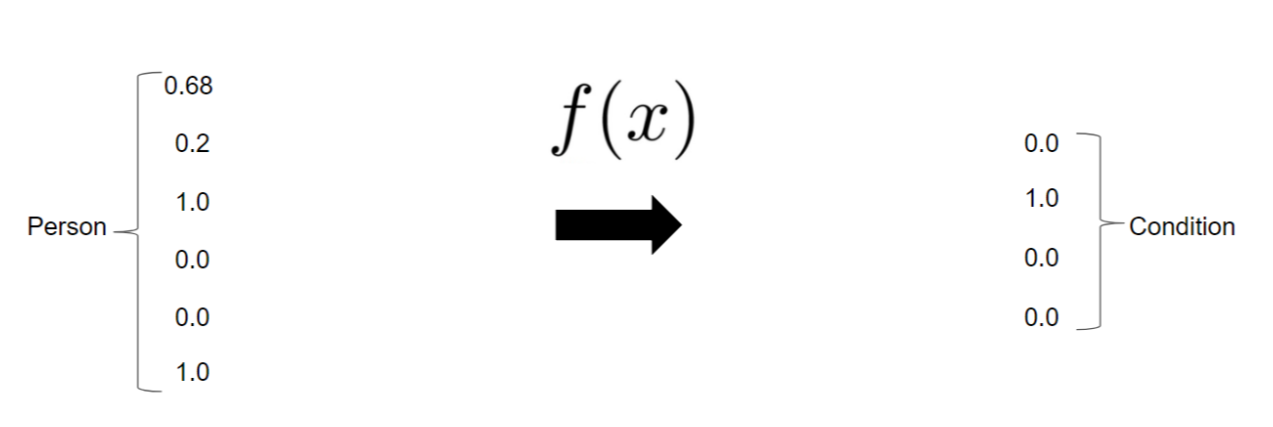
\includegraphics[width=\linewidth]{fgv.png}
	\end{center}
  \caption{Általános nézet}
\end{figure}

Ez így elég egyszerűen hangzik, mivel még nem tárgyaltunk arról, hogy ez a függvény hogyan működik, és honnan tud néhány adatból betegségre vonatkozó következtetéseket levonni. A kérdés tehát, hogy hogyan határozzuk meg ezt a függvényt. Legyen a függvény egy neurális háló (\ref{ab1.2}.~ábra).

\begin{figure}[h!]
 
 \begin{center}
	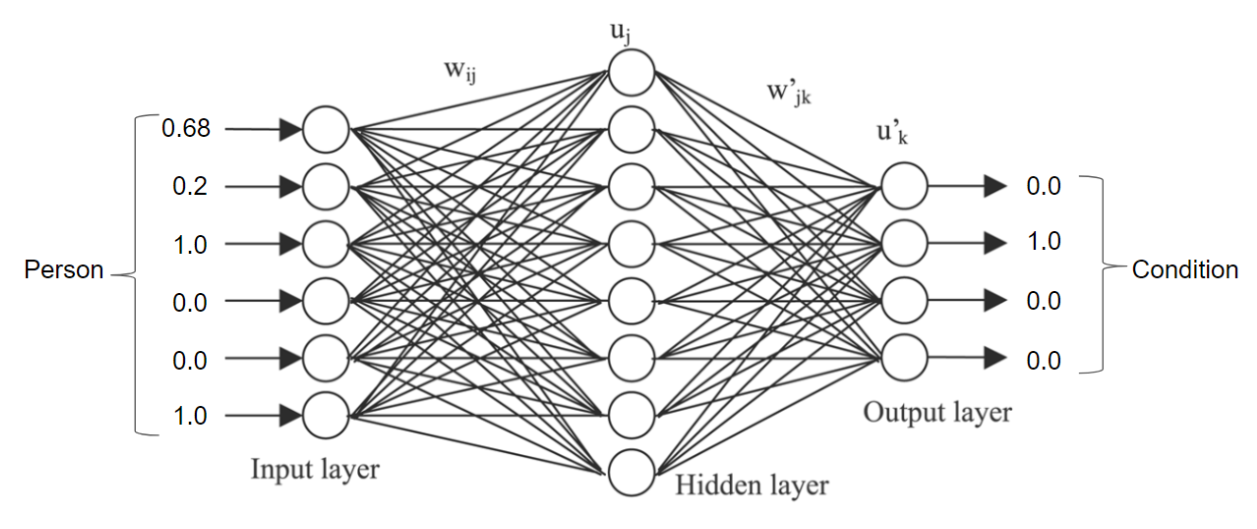
\includegraphics[width=.9\linewidth]{fgv_network.png}
 \end{center}

  \caption{Konkrét neurális háló}\label{ab1.2}
\end{figure}


A neurális háló tulajdonképpen egy súlyozott gráf (előrecsatolt háló), melynek $n$ darab csúcsa a bemeneteket reprezentálja, $k$ darab csúcsa pedig a kimeneteket. Az $n$ és $k$ csúcsok halmazát rendre input és output layernek (rétegnek) nevezzük, azonban a maradék csúcsok több kisebb halmazra bonthatóak, az úgynevezett hidden (rejtett) rétegekre. 

Egy egyszerű neurális háló tehát $L$ darab layerből áll, melyek közül az input és output layerek speciális funkciót látnak el. A rétegeknek van egy rögzített sorrendje, amely egy neurális hálónak fix tulajdonsága, sosem változik meg. Sorrendben az első réteg az input layer, amit néhány rejtett réteg követ, majd egy output layer zárja a listát.

Minden réteget neuronok egy halmaza alkot. Ezek a gráf csúcsai. Az élek kizárólag a szomszédos layerek neuronjai között futhatnak. A gráf összes éléhez tartozik továbbá egy-egy valós számértékű súly.

\begin{figure}[h!]
  
	\begin{center}
	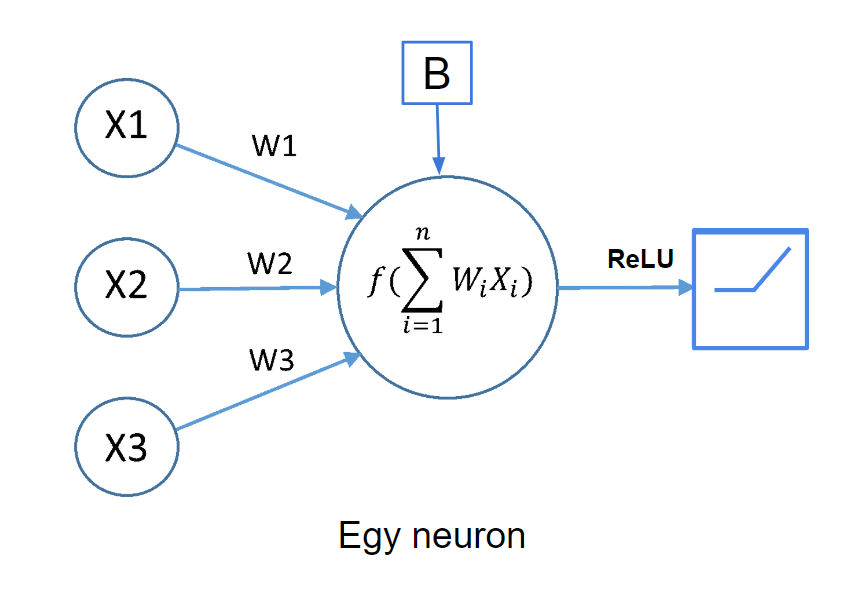
\includegraphics[width=.6\linewidth]{neuron.png}
	\end{center}
	
  \caption{Egy neuron}\label{ab1.3}
\end{figure}

A neuronoknak van egy úgynevezett aktivációs értékük, amely minden pillanatban az az érték, amelyet utoljára beállítottunk neki. Egy neuron aktivációs értéket úgy határozzuk meg, hogy vesszük a neuron rétegét megelőző layer azon neuronjait, amelyekkel össze van kötve, majd vesszük ezeknek a lineáris kombinációját a hozzájuk tartozó élek súlyaival. Ehhez még hozzáadunk egy bias értéket, amely magához a vizsgált neuronhoz tartozik és szintén egy tetszőleges valós szám.
Ezután még az így kapott összegre alkalmazunk egy úgynevezett aktivációs függvényt, amely ugyancsak a neuronhoz tartozik (bár általában egy rétegben ez minden neuronra azonos).
(\ref{ab1.3}.~ábra)


Az lineáris kombináció és a bias hozzáadása után keletkezett valós szám még nem az aktivációs érték lesz, hanem az aktivációs függvény értéke, ezen a helyen.
Többféle aktivációs függvény is használhatunk, a leggyakoribbak:

\begin{itemize}  
	\item Sigmoid: $f(x) = \frac{e^x}{e^x+1}$ 
	\item ReLU : $f(x) = max(0,x)$
\end{itemize}

Az input neuronoknál nem tudjuk kiszámolni a lineáris kombinációt, mivel nincs előző réteg, az ő esetükben egyenesen az aktivációs értéket állítjuk be inputnak. Miután minden input neuron aktivációs értékét beállítottuk látható, hogy az egész hálón végig fog menni egy változás, mert iteratívan minden réteget megelőző réteg megváltozik, tehát a maga a réteg is megváltozik.

Arra, hogy a neurális háló súlyai és biasei milyen értékek kezdetben, több lehetőség is van:
\begin{itemize}  
	\item mindegyik $0$ vagy mindegyik súly $1$
	\item valamilyen eloszlásból generált véletlen számok
	\item fájlból betöltött értékek (tanítás folytatása esetén)
\end{itemize}

Ha tehát megadunk egy inputot, akkor az meghatározza az output layer neuronjainak konkrét aktivációs értékeit. Ez az érték lista a függvény kimenete. Érezhető, hogy ha egyszerűen tetszőleges inputokra rá eresztjük ezt a kalkulációt, akkor az nagyjából véletlen outputokat fog generálni. A tanítás alapú mesterséges intelligencia algoritmusoknál azonban rendelkezésünkre állnak helyes input-output párok egy listája, vagyis egy inputhoz már kétféle outputot is tudunk mondani: az adathalmaz outputját, illetve ezt a véletlennek tűnő outputot amit a háló generál.

\begin{figure}[h!]
  
	\begin{center}
	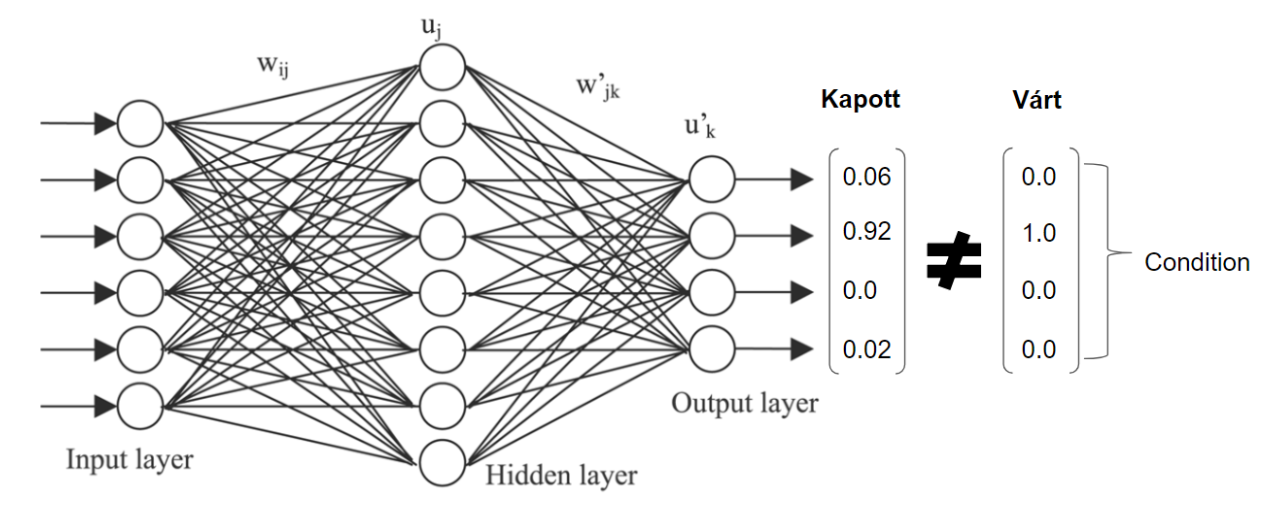
\includegraphics[width=\linewidth]{kapott_vart.png}
	\end{center}
	
  \caption{A kapott érték nem egyezik meg a várttal}
\end{figure}

Ha a hálónk, nem képes a várt kimenetet megközelíteni, akkor a mi megközelítésünkben hibázik. Olyan módon kell változtatni a neurális háló súlyait és biaseit, hogy ezek a hibák minimálisak legyenek, hiszen ekkor a predikció is pontos. Ennek megvalósításához elengedhetetlen, hogy a hibát számszerűsíteni tudjuk.

Azon függvényeket, melyek egy $t$ várt és egy $x$ kapott vektorhoz kiszámítanak egy hibát, $\lambda(x,t)$ veszteségfüggvénynek nevezzük.

\section{Backpropagation}

Minden input-output párra meg kell változtatni a súlyokat és biasokat, mindegyiket más mértékben. Minél jobban felelős egy súly a hibáért annál jobban meg kell azt változtatni. A felelősség eldöntéséhez backpropagáljuk a hibát, vagyis a hiba vektort aktivációs értékként beállítjuk az output layernek és fordított irányban végrehajtjuk a rétegek neuronjainak aktivációját.
Például: ha a hibavektor egyik neuronja $0$, tehát az adott értéket pontosan jósolta meg a háló, akkor a hozzá tartozó súlyoknak semmilyen felelőssége nincsen a hibában, ezért a $0$ érték propagálódik vissza rajtuk.

\begin{figure}[h!]
  
	\begin{center}
	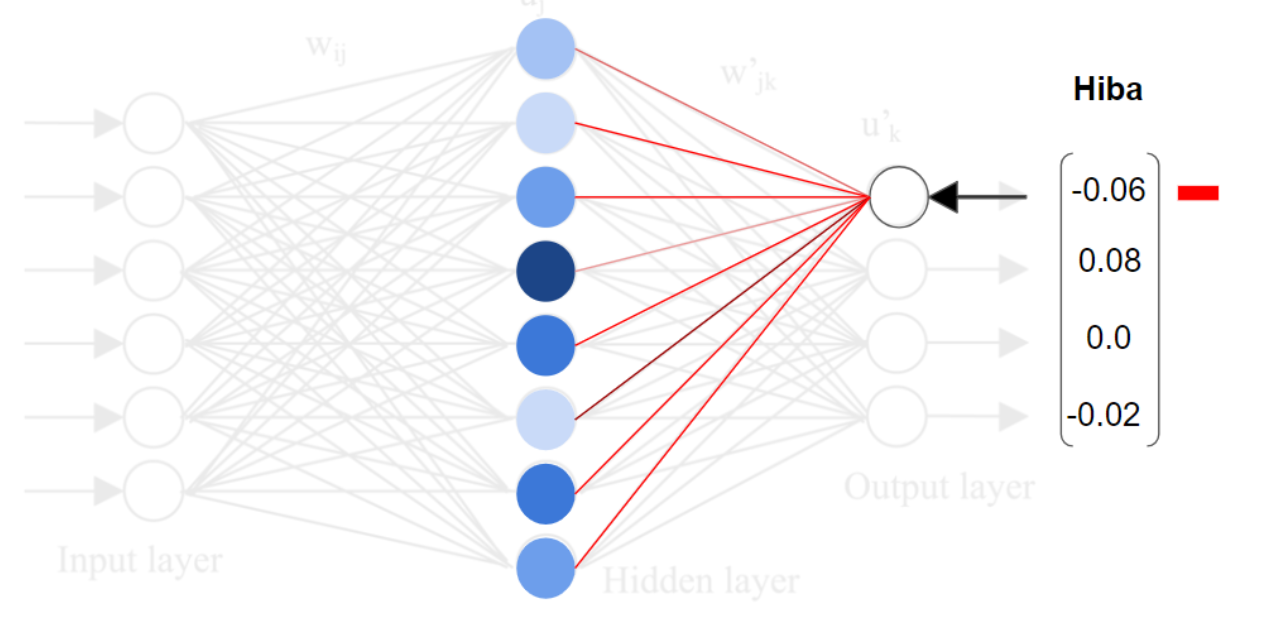
\includegraphics[width=.8\linewidth]{backprop_single_error.png}
	\end{center}
	
  \caption{Egy neuron felelőssége a mögötte lévő rétegben}
\end{figure}

A felelősséget végül nem a súlyokon, hanem a neuronokon fogjuk realizálni. A backpropagation végeztével tehát minden neuronon lesz egy felelősség érték.

\begin{figure}[h!]
  
	\begin{center}
	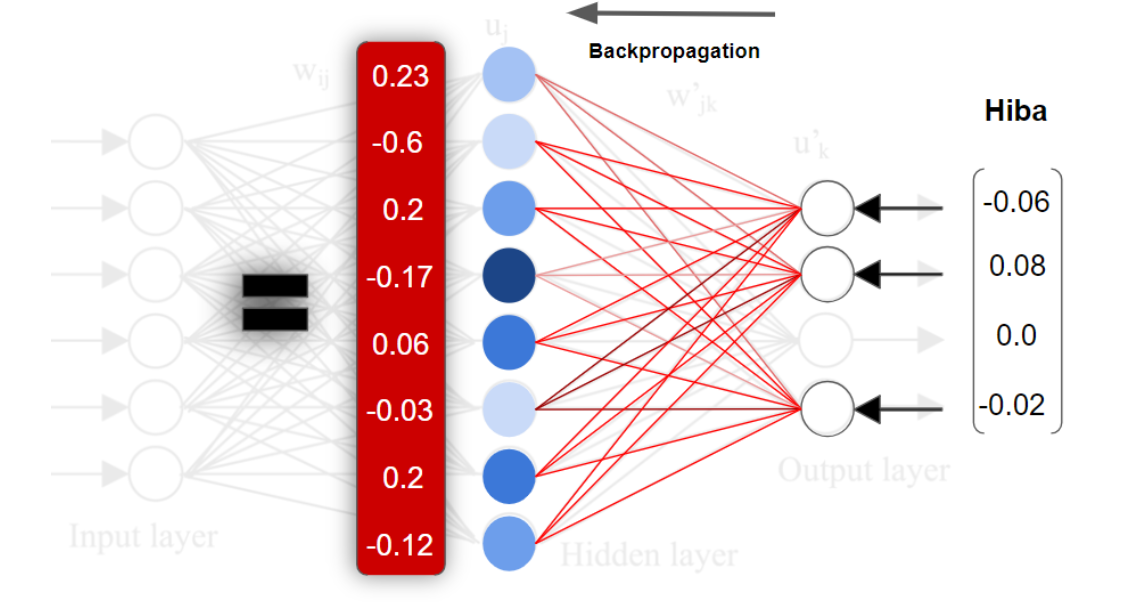
\includegraphics[width=.8\linewidth]{backprop_all_error.png}
	\end{center}
	
  \caption{Egy réteg teljes felelőssége a mögötte lévő rétegben}
\end{figure}

A neuronokon azonban nincs mit megváltoztatni, csak a súlyok és biasek változtatása lehetséges. A súlyok megváltoztatására a képlet az alábbi:
$$ w_{new} =  w_{old} + b_{act-error} \cdot f'(b_{act}) \cdot a_{act} \cdot lr $$
ahol $w$-vel jelölt értékekkel, a megváltoztatás előtti, illetve utáni súlyokat jelöljük, $a$ az (irányított) él kezdőpontja, $b$ pedig a végpontja (és $b_{act}$ az aktivációs függvény előtt értendő aktiváció), $lr$ pedig a tanulás sebessége. $b_{act-error}$ a backpropagation során kiszámolt neuron felelőssége a hibában, $f$ függvény pedig az aktivációs függvény (a képletben a deriváltja szerepel). 

A backpropagationt több input-output párra is el kell végezzük, ekkor viszünk be információt a rendszerbe arról, hogy mely párokat tartunk helyesnek, és végül az algoritmus ebből fogja ezt a véges tudását általánosítani bármilyen -- korábban nem látott -- inputra. Azt a folyamatot amikor az összes kívánt párra lefuttatjuk a backpropagationt \emph{epochnak} nevezzük. 

Ha általában meg szeretnénk mérni azt, hogy a jelenlegi háló milyen hatásfokkal tud prediktálni, akkor nem elég a tanítás közben megnézni, mekkora hibákat backpropagál program, mivel az egész háló arra van optimalizálva, hogy erre a konkrét tanító adathalmazra hatékonyan működjön. Éppen ezért a tanítás előtt két részre osztjuk az adathalmazt:

\begin{itemize}  
	\item tanító adatok (\emph{train set}): amelyeken végrehajtjuk a backpropagationt, 1 epochban minden adatra egyszer
	\item validációs adatok (\emph{validation set}): minden epoch végén leteszteljük ezekre az adatokra, hogy mekkora hiba keletkezik, backpropagationt viszont nem futtatunk a hibákon
\end{itemize}

A backpropagationt a gyakorlatban nem szokás minden egyes tanító adatpár után lefuttatni, hanem egyszerre több adatnak az aggregált hibáját vezetjük vissza a súlyok megváltoztatásához. Ez párhuzamosításra ad lehetőséget, amely nagy mértékben tudja csökkenteni a futásidőt.

Az epoch szám megválasztásánál figyelni kell arra, hogy a hálót ne tanítsuk túl (\emph{overfitting}), vagyis ne tanuljunk rá túl nagy mértékben a tanító adathalmazra, valamint ennek ellenkezője, az alul tanítás (\emph{underfitting}) is pontatlanságot eredményez, amikor egyszerűen a háló még a tanító adatokra sem képes megfelelő pontossággal predikálni.

\section{Konvolúciós hálók}

A konvolúciós hálókat \cite{ConvNet} a legtöbb esetben kép klasszifikációra használják, vagyis háló feladata az, hogy az inputjára kapott képről (egy előre meghatározott listából) eldöntse, hogy  mi szerepel rajta (például: kutya vagy macska). Ha $n$ féle osztályt klasszifikál a háló, akkor $n$ darab output neuronja van, a kép inputra adott válasza pedig egy $n$ elemű eloszlás arról, hogy a háló jelenlegi tudása szerint melyik osztály előfordulását milyen valószínűnek tartja.

A korábbiakban általánosságban tárgyaltuk a neurális hálókat, csak annyit állítottunk, hogy a szomszédos rétegek neuronjai vannak egymással kapcsoltan. Általános esetben egy réteg minden neuronja összeköttetésben áll az őt megelőző réteg mindenen neuronjával. Az ilyen réteget teljes-összeköttetésű rétegnek nevezik, a kizárólag ilyeneket tartalmazó hálók pedig sűrű (\emph{dense}) hálók.

Kép inputok esetén a sűrű hálók, azonban nem használják ki a képben rejlő azon információt, hogy bizonyos pixelek közelebb vannak egymáshoz mint más pixelek, hiszen az input neuronok szerepe a teljes-összeköttetés miatt felcserélhető. Egy sűrű hálónak ebben az esetben tehát még azt is meg kell tanulnia, hogy mit jelent képnek lenni (összefüggő egyszínű tartományok az egymáshoz közeli pixeleknél, néha éles színváltás).

Ezt a problémát oldják meg a konvolúciós hálók úgy, hogy nem kizárólagosan teljes-összeköttetésű rétegeket alkalmaznak, hanem egyéb speciális rétegeket is:

\begin{itemize}
  \item Konvolúciós réteg
  \item Pooling réteg
\end{itemize}

A konvolúciós hálók általában úgy vannak felépítve, hogy néhány konvolúciós rétegenként tartalmaznak egy pooling réteget, majd a kimeneti réteg -- amikor már csak egy $1$ dimenziós vektort várunk -- egy teljes-összeköttetésű réteg.

A súlyok javítására ugyanúgy a backpropagation algoritmus használjuk.

\subsection{Konvolúciós réteg}

A konvolúciós hálók rétegeit elsősorban három dimenziósnak képzeljük el. Színes kép esetén például az input réteg három dimenziója: a kép magassága, szélessége és a pixelek színe. A réteg példában szereplő szín dimenzióját a réteg mélységének nevezzük.

A konvolúciós rétegek $K$ darab szűrőből (filterből) állnak, melyek $n\times n$-es súly mátrixok, ahol $n$ általában egy kis egész szám, például 3, paraméter. Maga a réteg pontosan $K$ mélységű, minden filter egy alréteget határoz meg.

A réteg neuronjainak aktivációját a következőképpen számoljuk ki: az előző rétegnek vesszük az összes $n\times n\times d$-s ablakát, ahol $d$ az előző réteg mélységét, az ablak pedig egy neuronokból képezhető téglatestet jelöl, első réteg esetén például a középső $3\times3$ pixelt és színeiket. Minden ilyen ablak $K$ darab neuron aktivációját határozza meg, tehát minden filterhez egyet. A $k$-adik filter esetén az aktiváció az ablak neuron aktivációinak a filter súlyaival vett lineáris kombinációja lesz. Ezt hívják konvolúciónak.

\begin{figure}[h!]
\begin{center}
  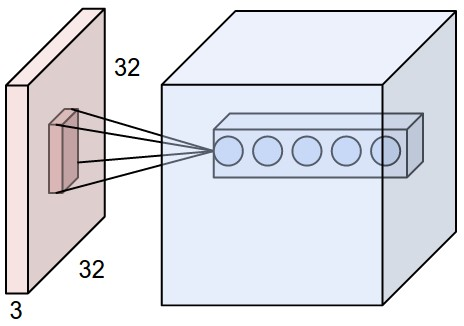
\includegraphics[width=0.4\linewidth]{depthcol.jpg}
  \caption{Egy konvolúciós réteg összes neuronja egy ablak pozícióhoz}
\end{center}
\end{figure}

Egy konvolúciós rétegnek vannak egyéb paraméterei is a filterek száma és az ablakméret mellett, például az hogy az ablak eltolásánál hány neuronnyit lépünk (\emph{stride}) vagy az ablak viselkedése a neuronmátrix határán (\emph{padding}), ezekkel azonban a dolgozat keretein belül nem foglalozunk.

\subsection{Pooling réteg}

Pooling rétegeket általában két konvolúciós réteg között szoktak használni a későbbi rétegek méretének csökkentése céljából. Ez csökkenti a súlyok számát, íg gyorsítja a futást, azonban ez a művelet információveszteséggel jár. Ha a képes analógiát tekintjük, ez egy veszteséges képméret csökkentésnek felel meg (lásd \ref{pool}.~ábra). A konvolúciós rétegeknél is (megfelelő padding típussal) csökken a méret, a pooling réteg esetében általában nagyságrendileg felezni szokás a szélességet és magasságot.

\begin{figure}[h!]
\begin{center}
  %\label{pool}
  
	\begin{center}
	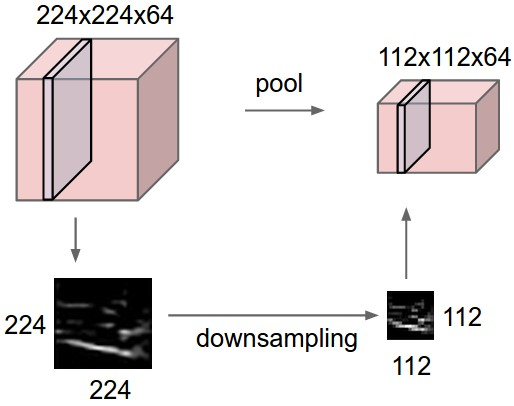
\includegraphics[width=0.5\linewidth]{pool.jpeg}
	\end{center}
	
  \caption{Egy konvolúciós réteg összes neuronja egy ablak pozícióhoz}\label{pool}
\end{center}
\end{figure}

\section{Autoencoderek}

Az autoencoderek olyan speciális neurális hálók, amelyek képesek az input rétegükre érkező adatot egy rövid kóddá tömöríteni (\emph{encode}), majd abból a kódból az eredeti inputot visszaállítani (\emph{decode}). Ezt a két funkciót egyetlen hálóval valósítjuk meg, azonban a hálón belül jól elkülönül a két rész: a rétegek első fele végzi el a kódolást, a második fele pedig a dekódolást. Az encodernek folyamatosan csökkennek, a decodernek pedig növekszenek a rétegeik mérete, ahogy ezt a \ref{AE_arch2}.~ábra mutatja. Az encode-olás és decode-olás egymás utáni elvégzése elméletben egy identitás. A tanítás során ezért a kimeneten várt érték maga az input, nincs szükségünk adatpárokra, pusztán kódolandó adatokra. A háló tanításához szükséges hibát tehát a rekonstrukció hatásfoka fogja meghatározni. A veszteségfüggvénye konkrétan az alábbi:

$$ \mathbb{E}_{q_\phi(z|x)} [\log p_\phi(x|z)]$$

Ez lényegében a várt és kapot vektorok távolság-négyzete, vagyis az input és output kép közíti négyzetes hiba. 

A háló ,,közepén'' elhelyezkedő legkisebb méretű réteget reprezentációs vagy látens rétegnek nevezzük, a kiértékelés során az itt megjelenő aktivációs értékek vektora jelenti a kódot. Ez a kód valóban az inputra érkező adatot reprezentálja, hiszen az adatból (az encoderrel) elő tudjuk állítani a kódot, a kódból pedig (a decoderrel) vissza tudjuk állítani az adatot.

A \ref{AE_arch2}.~ábrán látható input egy kép, az MNIST adathalmazból, mely nagy mennyiségű alacsony felbontású képeket tartalmaz rajzolt számjegyekről. Látható, hogy a (már előzőleg betanított) háló kis hibával, de képes rekonstruálni a képet (hiszen a kimenet valóban hasonlít a bemenetre). A kép vektor reprezentációja (kód) a középső két neuronjának aktivációjából olvasható ki. A háló (pontosabban a decoder) tehát képes volt 2 számból előállítani $784$ számot (egy $28\times 28$ pixel méretű képet), vagyis az autoencoderek nem csak kódolásra, hanem tömörítésre is alkalmasak.

\begin{figure}[h!]
\begin{center}
  
 
 \begin{center}
	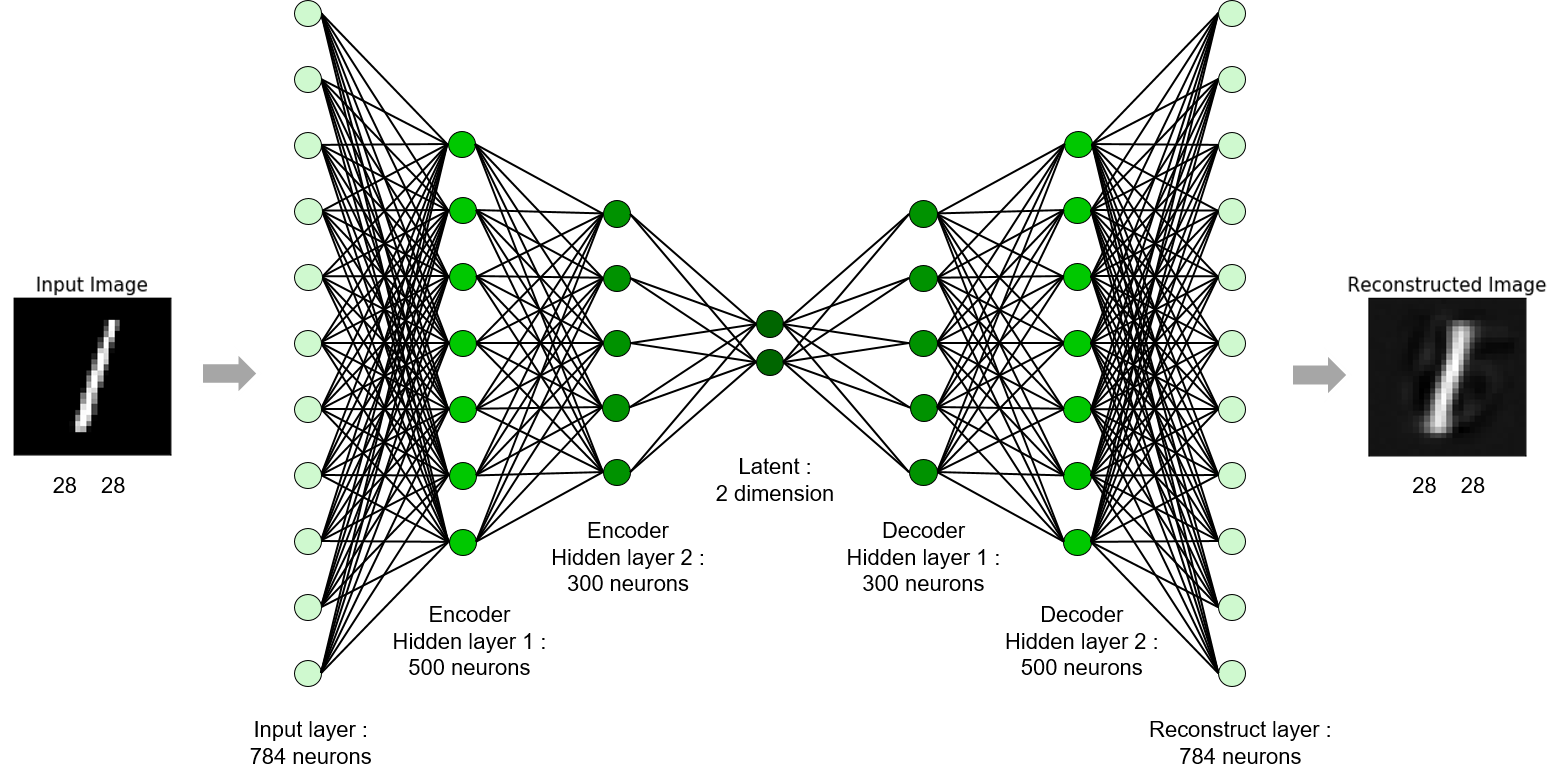
\includegraphics[width=\linewidth]{AE_arch2.png}
 \end{center}

  \caption{Autoencoder}\label{AE_arch2}
\end{center}
\end{figure}

\section{Generatív modellezés}

A generatív modellezés célja, hogy egy adott (címkézetlen) adathalmazból tanulva új adatokat tudjuk generálni ugyanazon eloszlásból, mint amelyből a tanító adatok származnak. Például ha macskákról készült képekkel tanítjuk a modellt, akkor az képes lesz új, korábban nem látott macskákat tartalmazó képeket generálni.

A gyakorlatban használt két legfőbb generatív modell architektúra:
\begin{itemize}
  \item Generative Adversarial Network (GAN)
  \item Variational AutoEncoder (VAE)
\end{itemize}

Jelenleg a GAN-ok a VAE-knél sikeresebb modellcsalád a generatív modellezés feladatára, de mi a dolgozatban a VAE-kre fogjuk helyezni a hangsúlyt, mégpedig azért, mert az autoencoder alapú modellek alkalmasabbak reprezentáció-tanulásra. A reprezentáció-tanulás fogalmát később fogjuk bevezetni, de röviden azt jelenti, hogy a hálózat képes automatikusan feltárni az adatainkban rejlő szabályszerűségeket.

\subsection{Generative Adversarial Network (GAN)}

A GAN-ok \cite{original GAN}, tehát ahogy korábban már említettük, olyan neurális hálózatok, melyek képesek az input adathalmaz eloszlásából újabb, véletlenszerű adatokat generálni. Ezt -- az autoencoderekhez hasonlóan -- két egymástól funkcionálisan eltérő neurális háló együttes használatával érjük el a GAN esetében. A két hálót \textit{generátornak} és \textit{diszkriminátornak} nevezzük.

A generátor feladata, hogy egy véletlenszerű kódból előállítson egy adatot az adathalmaz eloszlásából. A háló inputja tehát egy véletlen zaj, azaz minden input neuronnak egy véletlen értéket adunk meg mind tanításkor, mind kiértékeléskor. Már csak annyi a kérdés, hogy hogyan tudjuk eldönteni az output rétegén megjelenő generált adatról, hogy valóban a kívánt adathalmazból származik-e. Ezen eldöntendő kérdés megválaszolására használjuk a diszkriminátort. A generátor súlyait ezért annak függvényében változtatjuk, hogy a diszkriminátor milyen mértékben tartja valódinak az adatot.

A diszkriminátor feladata tehát, hogy egy adatról eldöntse, valóban az adathalmazból származik-e. Az inputja egy adat, az outputja pedig mindössze egy neuronból áll: amely az input hitelességének valószínűségét jelzi. A diszkriminátornak felváltva adunk adatokat az adathalmazból és a generátor kimenetéről, mindkét esetben tudjuk, hogy minek kell lennie a várt eredménynek ($0$ vagy $1$), így idővel megtanulja megkülönböztetni egymástól a valós és generált adatokat. 

A két hálót tehát párhuzamosan tanítjuk, a generátor folyamatosan megtanul adatokat generálni az adathalmaz eloszlásából, a diszkriminátor pedig folyamatosan megtanulja ,,leleplezni'' a generátort. A modell alapvető felépítését a \ref{gan}.~ábra szemlélteti.

\begin{figure}[h!]
\begin{center}
 
  
	\begin{center}
	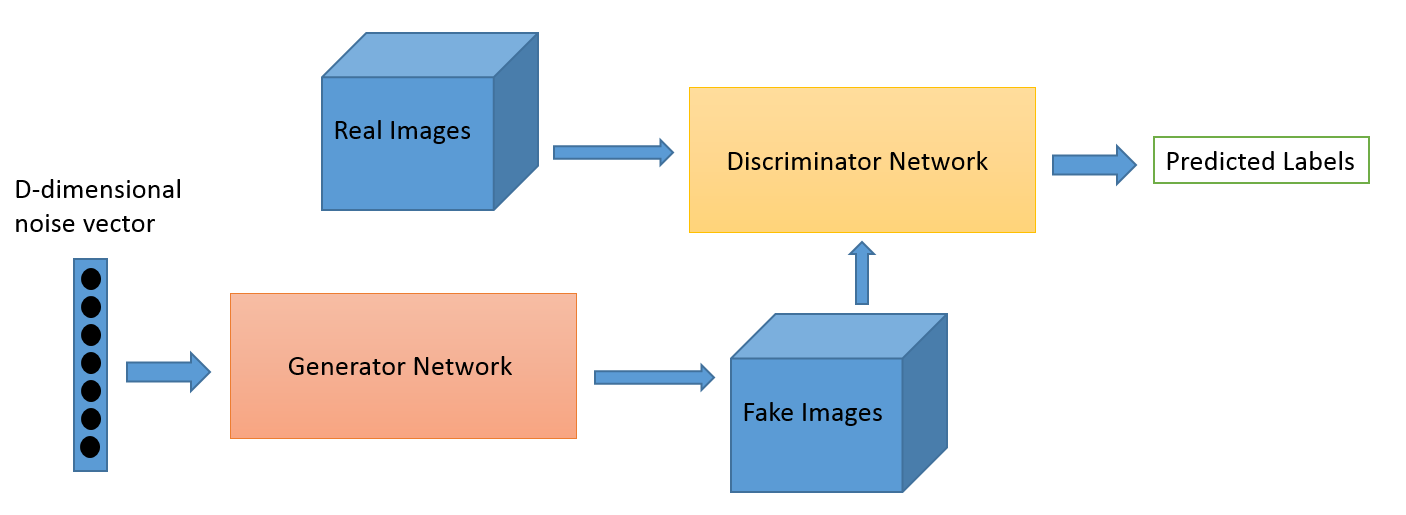
\includegraphics[width=\linewidth]{gan.png}
	\end{center}
	
  \caption{Generative Adversarial Network} \label{gan}
\end{center}
\end{figure}

Az utóbbi néhány évben nagy fejlődésen mentek keresztül a GAN-ok. A \ref{gan_progress}.~ábrán látható képeket a Celeba adathalmaz (amely híres emberek címkézett arcképeit tartalmazza) eloszlásából generálták GAN architektúrájú hálókkal. Jól látszik, hogy az elmúlt 5 évben mekkora fejlődésen ment keresztül a szakirány. 

\begin{figure}[h!]
\begin{center}
  
  
	\begin{center}
	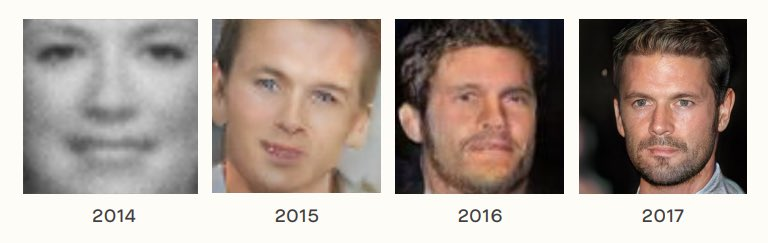
\includegraphics[width=\linewidth]{gan_progress.jpg}
	\end{center}
	
  \caption{GAN modellek fejlődése az elmúlt 4 évben}\label{gan_progress}
\end{center}
\end{figure}

\section{Variational Autoencoder (VAE)}

A variational autoencoderek a GAN-okhoz hasonlóan generatív modellek, azonban a felépítésük -- ahogy a nevükben is szerepel --  nagyban hasonlítanak a hagyományos autoencoderekhez.
Első ránézésre az autoencoderek is alkalmasnak tűnnek a generálásra, hiszen a decoder komponensük képes egy látens vektorból előállítani egy adatpontot, ezért ha egy korábban ismeretlen látens vektorra futtatjuk a decodert, akkor egy új, de mégis hiteles adatot kapnánk. Ez azonban nem működik, mert az autoencoder látens terében a gyakorlatban bizonyos térrészek teljesen érintetlenül maradnak, így a háló nincs felkészülve arra, hogy a látens tér azon szegmenséből generáljon (decode-oljon) adatot.

Ezt a problémát oldja meg a VAE \cite{original VAE} azzal a trükkel, hogy az encodere nem egy konkrét látens vektort állít elő, mint az adat reprezentációs alakja, hanem egy normális eloszlást. A variational autoencodereknél valójában ez az eloszlás reprezentálja az adatot, ami két vektort jelent: egy várható érték és szórás vektort, melyek koordinátánként értendőek a látens vektorra nézve. A tanítás során tehát a decoder (amit a VAE esetében már generátornak is nevezhetünk) inputja egy véletlenszerű vektor ebből az eloszlásból (lásd \ref{vae}.~ábra).

\begin{figure}[h!]
\begin{center}
  
  
	\begin{center}
	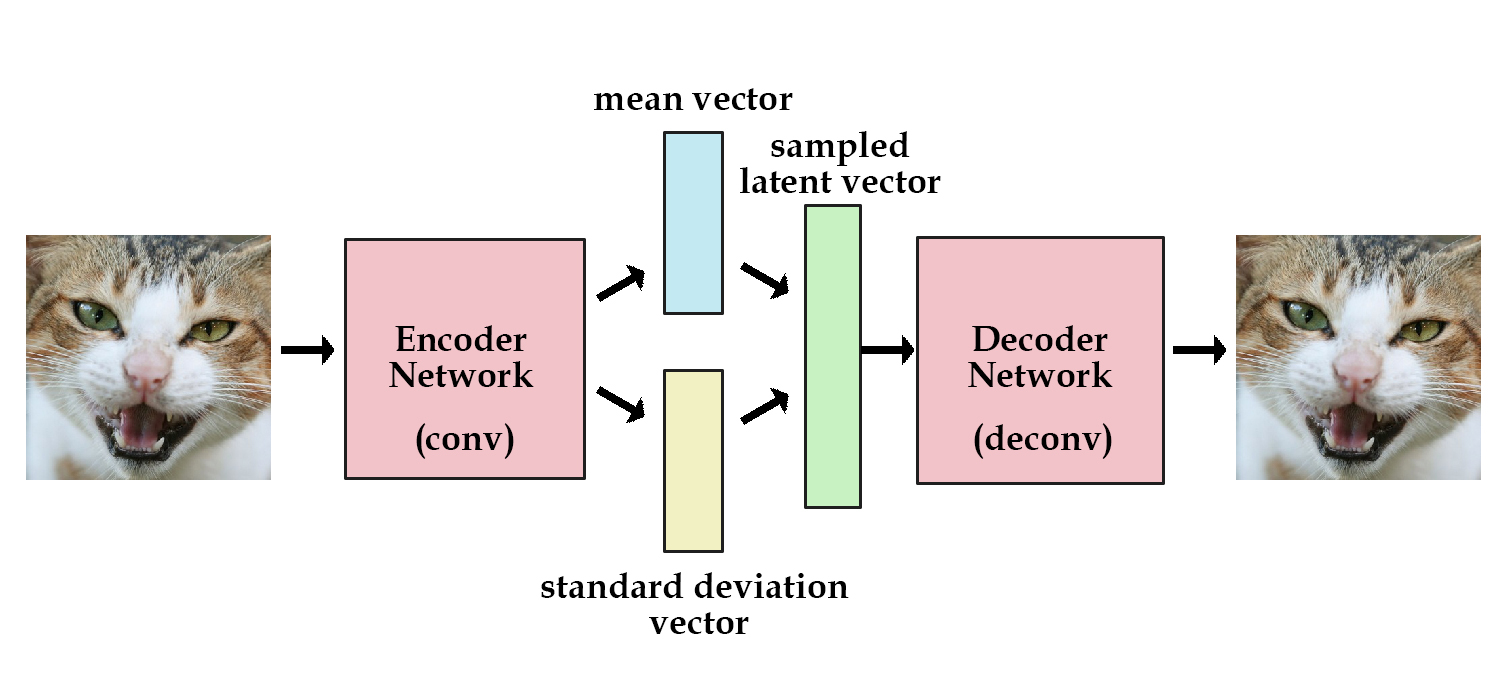
\includegraphics[width=\linewidth]{vae.jpg}
	\end{center}
	
  \caption{Variational Autoencoder működése}\label{vae}
\end{center}
\end{figure}

A VAE-k másik fő eltérése a hagyományos autoencoderektől, hogy a backpropagation során nem pusztán a rekonstrukció sikeressége szerint javítják a háló súlyait, hanem az KL (Kullback–Leibler) divergencia függvényében is. A KL divergencia nem a kimeneten kapott adatot minősíti, hanem azt, hogy a létrejött eloszlások hogyan helyezkednek el a látens térben. Röviden: az olyan eloszlás halmazokat jutalmazza, amelyek egyenletesen fedik le a látens teret. A tanítás során ezért az adathalmaz adataihoz párosítható látens reprezentációk az egész teret lefedik.

A hagyományos VAE hálók veszteségfüggvénye az alábbi:
$$ \mathbb{E}_{q_\phi(z|x)} [\log p_\phi(x|z)] + D_{KL}(q_\phi(z|x)||p_\phi(z))$$

Ebben a veszteségfüggvényben a korábbi rekonstrukciós tag mellett megjelenik a KL divergencia is.

A tanítás végeztével tehát a látens térből bárhonnan választhatunk véletlen vektorokat, azokból valósághű adatotokat fog generálni a decoder.

\section{Módosított variational autoencoderek ($\beta$-VAE)}

A $\beta$-VAE-k \cite{bvae} nagyon hasonlóak a rendes VAE hálókhoz, mindössze a veszteségfüggvényben különböznek egymástól. A VAE-k esetében ez a veszteség két komponensből áll: a rekonstrukciós veszteségből és a KL divergenciából. A $\beta$-VAE-ben szereplő béta mindössze egy konstanst jelent, amely azt határozza meg, hogy a teljes veszteség kiszámításnál a két komponenst milyen súllyal számoljuk, egészen konkrétan a rekonstrukciós veszteségnek mindig $1$, a KL divergenciának pedig $\beta$ a súlya. A veszteségfüggvény tehát egy $\beta$ szorzóval egészül ki az alábbi módon:
$$ \mathbb{E}_{q_\phi(z|x)} [\log p_\phi(x|z)] + \beta D_{KL}(q_\phi(z|x)||p_\phi(z))$$
A rendes VAE hálók tehát valójában $\beta=1$ paraméterű $\beta$-VAE-k.

A rekonstrukciós veszteség és a KL divergencia két egymásnak ellentétes erőhatásként képzelhető el a látens tér pontjaira nézve, ahol a rekonstrukciós veszteség célja az, hogy a pontok minél inkább távolodjanak az origótól (ezért egymástól is), így könnyebben megkülönböztethetőek legyenek a generálásnál, a KL divergencia pedig éppen az origó felé mozgatja azokat, hogy a térben kevés olyan térrész legyen ami betöltetlen. A $\beta$ paraméter ennek a két tendenciának az egymáshoz viszonyított erősségét szabályozza.

A gyakorlati tapasztalat azt mutatja, hogy a $\beta$ paraméter növelése javítja a látens tér reprezentációját, cserébe viszont rontja a rekonstrukciót.

\chapter{A feladat leírása}

A dolgozatban különböző VAE implementációkat tesztelünk egy bizonyos Dsprite adathalmazon (lásd később). Megvizsgáljuk, hogy a háló különböző paramétereinek változtatása, mint például (tanítási ráta, látens tér dimenziója, béta hiperparaméter) milyen hatással van a veszteségfüggvényekre és a rekonstrukcióra.

Az modellek strukturáltságát a Dsprite adathalmazban szereplő képek alakzatainak eltolása alapján vizsgáljuk. Különböző metrikákat hozunk létre és tesztelünk egy adathalamaz látens térben való leképzéséből kapott reprezentáció strukturáltságának számszerűsítésére. Ezen metrikák függését megvizsgáljuk a korábban említett paraméterektől különös hangsúlyt fektetve a $\beta$ hiperparaméterre ($\beta$-VAE) esetén.

A vizsgálatokhoz szükséges kiértékelő programokat Kerasban, Python nyelven, a legnépszerűbb gépi tanulás könyvtárakat felhasználva implementáljuk. Az eredmények megjelneítéséhez szükséges grafikonokat legeneráljuk a kiértékelő kimeneteit felhasználva.

\section{Dsprite adathalmaz}

A kísérletekhez használt adatokat a Dsprite \cite{Dsprite} adathalmazból vesszük, mely a GitHubon szabadon elérhető, letölthető.

A Dsprite egy úgynevezett szintetikus adathalmaz, ami azt jelenti, hogy az adatai nem a valóságból származnak, hanem külön erre a célra lettek legenerálva egy másik programmal. Maguk az adatok egészen pontosan $64\times64$ pixel felbontású képek, melyeken különböző alakzatok sokféle elforgatásban, eltolásban és méretben szerepelnek. Az adathalmaz továbbá címkézve is van, tehát minden képhez tartozik a rajta szereplő alakzat pontos leírása, egészen konkrétan:

\begin{itemize}
  \item típus: az alakzat formája ($3$ féle lehet: négyzet, ellipszis, szív)
  \item méret: az alakzat mérete ($6$ féle lehet)
  \item orientáció: az alakzat elforgatottságának mértéke ($40$ féle lehet)
  \item pozíció: az alakzat elhelyezkedése x és y irányban ($32\times32$ féle lehet)
\end{itemize}

A Dsprite ezen attribútumok összes lehetséges kombinációját tartalmazza, tehát az adathalmaz pontosan
$$ 3\cdot6\cdot40\cdot32\cdot32= 737280$$
darab adatot tartalmaz. A \ref{samples} táblázatban látható néhány minta az adatok közül.

\begin{figure}[h!]
\begin{center}

\begin{tabular}{| m{2.5cm} | m{2.5cm} | m{2cm}  | m{2cm} |  m{2.5cm} |}
\hline
Kép/Adat & Alak & Méret & Orientáció & Pozíció $(x,y)$ \\
\hline\hline
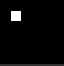
\includegraphics{sample00000.png} & $1$ (Négyzet) & $1$ & $1$ & $(1,1)$ \\
\hline

\includegraphics{sample0051616.png} & $1$ (Négyzet) & $1$ & $6$ & $(17,17)$ \\
\hline

\includegraphics{sample1001616.png} & $2$ (Ellipszis) & $1$ & $1$ & $(17,17)$ \\
\hline

\includegraphics{sample1501616.png} & $2$ (Ellipszis) & $6$ & $1$ & $(17,17)$ \\
\hline

\includegraphics{sample2003131.png} & $3$ (Szív) & $1$ & $1$ & $(32,32)$ \\
\hline
\end{tabular}
\end{center}
\caption{Példák a Dsprite adathalmazból}\label{samples}
\end{figure}

Ezen a ponton felmerülhet a kérdés, hogy miért foglalkozunk azzal, hogy az adatok mellé milyen extra információ (címke) párosul az adathalmazban, amikor korábban már láttuk, hogy az autoencoderek és VAE-k esetén pusztán a címkézetlen adatokat használjuk. Valóban, sem a hálók tanításhoz, sem a kiértékelésükhöz nem fogjuk használni ezeket a csatolt tulajdonságokat, a látens tér struktúráltságának méréséhez azonban igen, mivel a dolgozatban nem csupán adatokat generálunk a megadott adathalmaz eloszlásából, hanem szeretnénk megérteni a létrejött látens teret is.

\section{Reprezentáció tanulás}

A reprezentáció tanulás célja, hogy egy olyan látens ponthalmazzá képezze le az adathalmazt, amely elősegíti az adatok rejtett attributumainak feltárását. Erre különösen akkor van szükség, ha az adathalmaz címkézetlen. Ha például az adathalmazunk kutyákat és macskákat ábrázoló képekből áll, akkor a cél az, hogy a háló látens terében jól elkülönüljenek egymástól a két állatfajhoz tartozó látens reprezentációk.

A dolgozatunkban az a célunk, hogy az adathalmazból kinyerjük a képeken található alakzatok geometriai pozíciójára vonatkozó "rejtett" (mivel a címkéket nem használjuk a tanításhoz) információt, vagyis, hogy a hálónk olyan látens reprezentációkat hozzon létre a különböző képekhez, amelyekből következtethetünk a pozícióra.

\section{Disentanglement}

A disentanglement feladata az, hogy a reprezentáció tanulás során felismert attributumok a lehető legegyszerűbben formában jelenjenek meg a látens térben. Az ideális cél az, hogy minden látens neuron pontosan egy adat-tulajdonságért feleljen. Ebben az esetben, ha egy neuron értékét változtatjuk, akkor az kizárólag a hozzá tartozó tulajdonságot változtatja a generált adatban.

A mi esetünkben az alakzatok $x$ és $y$ koordinátáját szeretnénk szétválasztani, amennyiben egy alakzat összes lehetséges eltolásából képzett látens teret vizsgáljuk.

\chapter{Megvalósítás}

\section{Az alkalmazott szoftverarchitektúra ismertetése}

A matematikai és egyéb kutatási irányok esetén gyakran használják a Python programnyelvet, így van ez a neurális hálóknál is. Gyakorlati alkalmazás (például egy Androidos arcfelismerő) esetén természetesen már más nyelveket is szoktak használni, a mi programunknak azonban nincsen semmilyen közvetlen gyakorlati haszna, pusztán kutatási célokat szolgál.

A szoftverünkben felhasznált neurális hálókat kezelő könyvtárak a TensorFlow \cite{tensorflow} és a Keras \cite{Keras}, melyek nem egymástól függetlenül, hanem egymás segítve működnek, mivel a Keras egy magasabb szintű réteg, amely egy egyszerűbb interfészt nyújt a felhaszánló felé, és használja a Tensorflow-t. A programban használt főbb programcsomagok és verzióik a következőek:

\begin{itemize}
  \item Keras (2.2.2)
  \item Keras-Applications (1.0.4)
  \item Keras-Preprocessing (1.0.2)
  \item matplotlib (2.2.3)
  \item numpy (1.14.5)
  \item scipy (1.1.0)
  \item scikit-learn (0.19.2)
  \item tensorboard (1.10.0)
  \item tensorflow-gpu (1.10.1)
\end{itemize}

Ezek egyszerű, magas-szintű hozzáférést biztosítanak a hálókhoz, ezért nem kell külön megírni például a backprogpagation algoritmust, csak meghívni az alábbi metódust:

%\lstset{language=Python}
\begin{python}
model.fit(train_data,train_data)
\end{python}

Természetesen megadható számos paraméter a tanító adatpárokon kívül, például a epoch szám, vagy a batchek mérete. Észrevehetjük, hogy a fenti függvényhívás mindkét paramétere a tanító halmaz. Ennek az a magyarázata, hogy a hálónk egy (variational) autoencoder, tehát a tanítás célja a rekonstrukció, azaz akkor tekintjük az eredményt a legjobbnak, ha a kimeneten ugyanazt látjuk mint a bemeneten. Egy klasszifikáló háló esetében például az első paraméter az adatok, a második pedig a hozzátartozó címkék lennének.

A keretrendszer úgy van kialakítva, hogy a hálók alapvető paramétereit (epoch szám, batch méret, látens tér mérete, $\dots$) a programkód változtatása nélkül, egy külön (.ini kiterjesztésű) fájlból változtathatjuk. Egészen konkrétan a program kiinduló pontját jelentő generative.py programot egyetlen argumentummal, egy .ini fájlhoz vezető úttal kell meghívni. Alább látható egy példa egy adott paraméterezésű háló betanítására:


\lstset{language=sh}
\begin{python}
python generative.py vae.ini
\end{python}

Itt tehát a \pythoninline{vae.ini} fájl minden információt tartalmaz a tanítandó hálóról, az adathalmaz is linkelve van benne. Egy ilyen paraméter fájl ezért pontosan leír egy kísérletet, utólag is megtekinthető (készül róla egy másolat is, ami a betanított háló fájljai mellé kerül). Itt látható példa egy kísérletre (.ini fájlra):

\begin{python}
activation	relu
batch_size	50
color	False
dataset	dsprite
encoder	conv_deconv
encoder_conv_channels   32,32,32
encoder_use_bn	False
encoder_wd	0.0
frequency	2
generator	conv_deconv
generator_conv_channels   32,32,32
generator_use_bn	False
generator_wd	0.0
ini_file	[]
latent_dim	10
loss_generator  mse_loss
loss_encoder    size_loss,variance_loss
lr	0.0003
memory_share	0.45
metrics	mse_loss
model_type	autoencoder
nb_epoch	15
optimizer	adam
outdir	pictures/beta_vae_tuned
sampling	True
shape	64,64
testSize	10000
trainSize	727200
verbose	2
weights size_loss|1,variance_loss|1
\end{python}


\subsection{Az általunk vizsgált paraméterek ismertetése}

\begin{itemize}
  \item Tanítási idő (\pythoninline{nb_epoch}): A teljes tanító adathalmazon annyiszor tanítjuk be a hálót, amennyi az epoch-ok száma, ahol a tanítást minden epoch-nál onnan folytatjuk, ahol az előző epoch befejezte. Azért van szükség egynél több epoch-ra, mert a tanítási rátát szándékosan alacsonyra állítjuk, ezért a súlyoknak többszöri frissítésre van szükségük, hogy elérjék az optimumot.
  \item Tanítási ráta (\pythoninline{lr}): Annak a mértéke, hogy a súlyokat milyen mértékben változtatjuk ahhoz képest, hogy a backprogapation szerint mennyit kéne csökkenteni rajtuk az adott pillanatban. Ha a súly változtatás függvénye csak $w_{new} =  w_{old} + b_{act-error} \cdot f'(b_{act}) \cdot a_{act}$ lenne, akkor minden alkalommal túl sokat javítanánk a súlyokon, és a veszteségfüggvény értéke nagyon lassan csökkenne, vagy akár divergálna (lásd. \ref{para}.~ábra). Ezért kell a végén alkalmazunk még egy $lr$ tényezőt.
  \item Súly felejtés (\pythoninline{encoder_wd} és \pythoninline{decoder_wd} (weight decay)): Minden batch-ben ezzel a mértékkel csökken az összes súly értéke. Minél nagyobb az értéke annál jobban segíti a háló regularizációját (az output mennyire érzékeny az input kismértékű megváltozására). Képek esetén például általában nem kívánatos működés, ha az input egy pixelének változása óriási változást eredményez az outputon. Külön-külön beállítható az encoderre és decoderre.
  \item $\beta$ hiperparaméter  (\pythoninline{weights}): A rekonstrukciós veszteség tag és KL divergencia szignifikanciájának aránya.
  \item Látens tér dimenziója (\pythoninline{latent_dim}): Az autoencoder szűk keresztmetszetének mérete. Egy ilyen dimenziós térben kell végül reprezentálni az adatokat, ahonnan a rekonstrukció történik majd.
  \item Háló architektúrája (\pythoninline{encoder} és \pythoninline{decoder}): A háló felépítésének típusa. Korábban tárgyaltunk erre két lehetőséget: a Sűrű és Konvolúciós hálókat.
\end{itemize}

A tanítás végeztével az eredmények a keretrendszer működése szerint az .ini fájlban megadott \pythoninline{outputdir} mappába kerülnek (a fenti példában \pythoninline{pictures/beta_vae_tuned}). Ebben a directoryban a program a reprodukálhatóság és visszakövethetőség érdekében elmenti a tanítás összes hiperparaméterét egy (\pythoninline{all_params.ini}) .ini fájlban. Eltáródik továbbá magának a hálónak az architektúrája az \pythoninline{encoder.json} és \pythoninline{generator.json} fájlokban (közvetlenül ezt használja a program egy háló beolvasásához). Természetesen azt is el kell menteni, hogy mi lett a tanítás eredménye, vagyis a háló éleinek végleges súlyait. Ezeket a \pythoninline{encoder.h5} és \pythoninline{generator.h5} fájlokban tároljuk el. A háló utólagos kiértékelése és korábban ismeretlen adatokra futtatása esetén a program ezekből a fájlokból olvassa be és építi fel a hálót.

Ezeken az alapvetően szükséges fájlokon kívül a mi programunk kiment egyéb -- a tanítás hatékonyságát szemléltető -- kép fájlokat is. Ez néhány epochonként történik meg.

Az egyik ilyen fájl a \pythoninline{train_<epoch>.png}, amely néhány véletlenszerűen kiválasztott input/output párt rajzol ki az adott epochban. Egy ilyen kép látható a \ref{trainpng}.~ábrán (párosával vannak: bal oldalon az input, jobb oldalon az output).

\begin{figure}[h!]
\begin{center}
  
  
	\begin{center}
	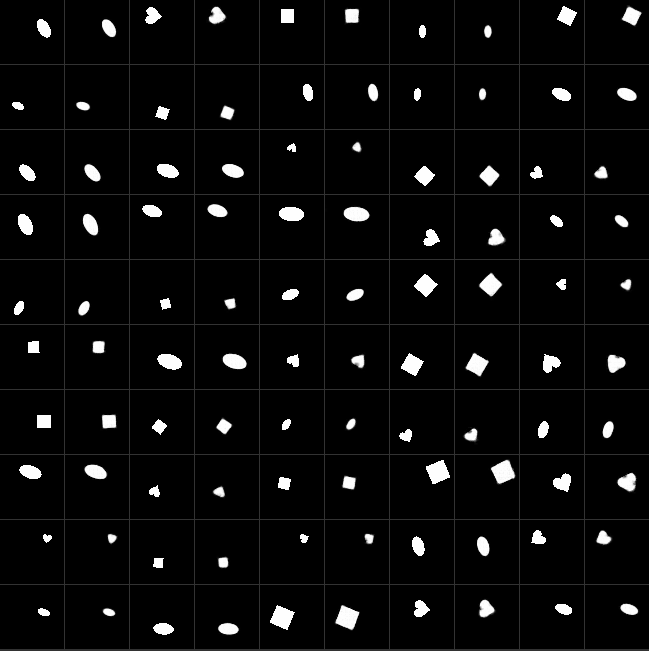
\includegraphics[width=0.75\linewidth]{trainpng.png}
	\end{center}
	
  \caption{Input/Output párok a tanítás során}\label{trainpng}
\end{center}
\end{figure}

A \pythoninline{test_<epoch>.png} kép nagyban hasonlít a \pythoninline{train_<epoch>.png}-hez, azonban itt csak a tesztelési adatokra adott kimeneteket nézzük, tehát a \ref{testpng}.~ábrán látható adatokat nem tanítottuk meg a hálónak. Egy autoencoder esetében természetesen az elvárás éppen az, hogy olyan adatokra is képes legyen rekonstruálni, melyet korábban nem látott.

 \begin{figure}[h!]
\begin{center}
  
  
	\begin{center}
	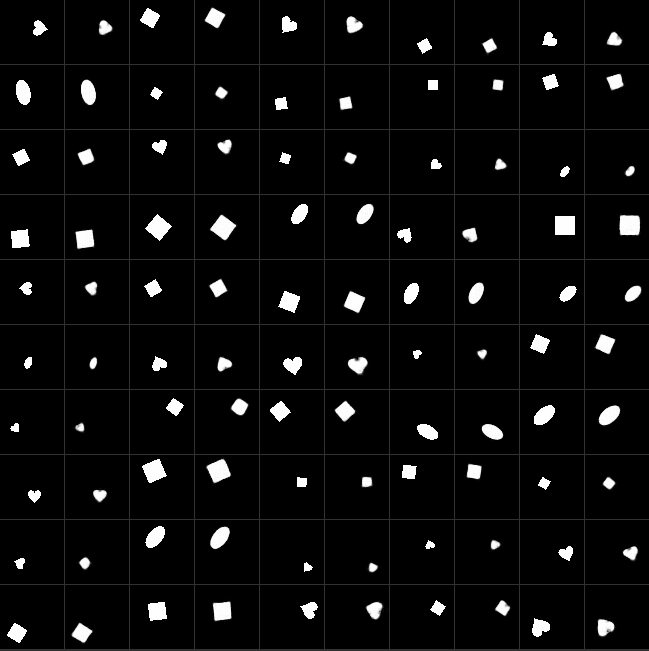
\includegraphics[width=0.75\linewidth]{testpng.png}
	\end{center}
	
  \caption{Input/Output párok a teszt adathalmazon}\label{testpng}
\end{center}
\end{figure}

Az iménti két képen a háló autoencoder jellegét validálhattuk szemrevételezéssel, azonban a mi hálónk egy VAE, tehát a betanítás után képes újabb képeket generálni anélkül, hogy egy input adatot adnánk neki. Ilyen, véletlen látens vektorokból generált képeket tárolunk el a \pythoninline{random_<epoch>.png} fájlban (lásd \ref{randompng}.~ábra). Ezen a képen már nem párokban vannak az adatok, minden szegmens egy különböző látens vektorhoz tartozik.

\begin{figure}[h!]
\begin{center}
  
  
	\begin{center}
	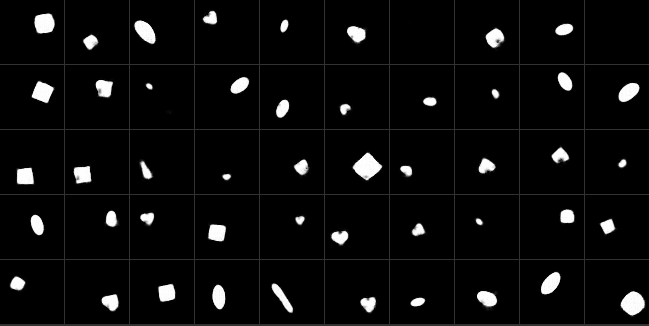
\includegraphics[width=0.75\linewidth]{randompng.png}
	\end{center}
	
  \caption{Véletlenszerűen sorsolt látens vektorokból generált képek}\label{randompng}
\end{center}
\end{figure}

\subsection{Eredmények feldolgozása és kiértékelése}

Az eddigiekben bemutatott keretrendszert az MTA Rényi Alfréd Matematikai Kutatóintézet munkatársai készítették, a dolgozatban prezentált eredmények előállításához mindössze eszközként használtam.

A saját kontribúcióm többek között a Dsprite adatbázis integrálása volt a keretrendszerbe, amelyhez egy mintavételező programot is írtam, hogy a tanításhoz szükséges adatmennyiséget csökkentsem, erre azonban végül nem volt szükség, mert a hálót nem terhelte meg nagyon (nem tartott sokáig a tanítás) a teljes adathalmaz sem, habár ehhez az epoch számot csökkenteni kellett. 

Az általam írt kód nagy része azonban egy külön Python fájlban (\pythoninline{lookup.py}) található, amely a későbbiekben tárgyalt metrikák kiszámolását végzi. Ehhez feldolgozza az adathalmazt és lehetőséget nyújt az adatok igény szerinti elérésére, például képes visszaadni egy paraméterben megadott típusú, eltolású, orientációjú és méretű alakzatot árbázoló képet, amelyhez az adathalmaz felépítéséből adódóan nincs szükség keresésre, explicit kiszámolható az adathoz tartozó index. Ezt felhasználva képes visszaadni egy alakzathoz az összes lehetséges eltolását is, amit közvetlenül a metrikák kiszámolásához használ fel.

A program továbbá be tud olvasni a fent említett fájlokból korábban betanított modelleket, és ezeket ki is tudja értékelni az adathalmazból kiválsztott különböző részhalmazokon. A háló futtatásának végeredményét, többek között a különböző veszteségeket  a konzolra írja ki (amelyet egy log fájlba mentünk a program futtatása közben). Ehhez hasonlóan a futtatás közben generálódó látens ponthalmaz alapján képes meghatározni a metrikáinkat, melyeket ugyanúgy a konzolra iratunk ki. A kísérleteknél látható veszteségfüggvények pontjai egy-egy ilyen kiemenetből származnak, egy ilyen grafikont több háló határoz meg, ezért ezeket egy külön programmal (\pythoninline{graph.py}) összegzünk, majd rajzounk ki. Azon grafikonokat melyek egy-egy hálót jellemeznek (mint például a \ref{m3D} vagy \ref{b4-splice}.~ábrák), azonban ez a program rajzolja ki.

A kísérletek elvégzéséhez számos hálót kellett betanítani, amit nem egyesével tettem meg, hanem bash scriptekkel automatizáltam a hálók egymás után való tanítását. Ennek működése az \pythoninline{.ini} fájlok (melyek egyértelműen leírnak egy hálót) paramétereinek változtatásán alapszik. Egy script legenerálja az összes háló \pythoninline{.ini} fájlját, majd egy másik script végig iterál az összesen és mindegyik alapján elkészít és betanít egy hálót (a \pythoninline{lookup.py} pedig ezeken a betanított hálókon fut). 


\subsection{Futásidő}

A neurális hálók tanítás általánosságban véve egy lassú folyamat, azonban (a batchek használata miatt) lehetőség nyílik nagymértékű párhuzamosításra, ezért a legtöbb esetben grafikus kártyákat használnak erre a célra. A dolgozatban prezentált hálókat is mind GPU-kon, Nvidia GTX 1080 Ti kártyákon tanítottam, melyekhez az MTA Rényi Alfréd Matematikai Kutatóintézet biztosított hozzáférést. Ezek jelenleg a legnagyobb teljesítményű magáncélokra gyártott grafikus kártyák közé tartoznak, azonban egy-egy háló betanítása így is megközelítőleg 1 óráig tartott rajtuk. Ez a futásidő a Kísérletek fejezetben bemutatott hálókra volt általánosságban jellemző.

\section{Látens reprezentációk strukturáltságának\\ számszerűsítése}

Egy variational autoencoderrel, amivel dolgozunk, képesek vagyunk az input adathalmaz eloszlásából véletlen adatokat generálni. Ez a VAE hálók rendeltetésszerű működése. A mi célunk az, hogy az alakzatokon végzett transzformációk a látens térben is strukturált módon jelenjenek meg.

Ezen a ponton használjuk fel az adathalmaz címkéit, tehát hogy valójában minden képhez ismerjük a rajta szereplő alakzat összes transzformációját (pozíció, méret, forgatás). Az adathalmazból így ki tudjuk keresni az összes olyan képet, melyen egy alakzat, egy forgatásban és egy méretben szerepel, vagyis annak az alakzatnak az összes eltolását. Ezt az összesen $32\times32$ adatból álló képhalmazt nevezzük $Q$-nak. A következőkben azt vizsgáljuk, hogy azon vektorok a látens térben, melyekből ezek a képek generálódnak, hogyan helyezkednek el.

Az alakzatok összes lehetséges eltolását két egymástól független paraméterrel le tudjuk írni: az $x$ és $y$ pozíciókkal. Azt szeretnénk látni, hogy ezen képek látens vektorai is leírhatóak két koordinátával a látens térben. Az ideális természetesen az lenne, ha a látensvektor egy-egy koordinátája egy az egyben megfeleltethető lenne $x$-nek és $y$-nak, azonban ezt nehéz feladat kikényszeríteni. Csak annyit valósítunk meg, hogy $Q$ halmaz egy olyan strukturált ponthalmazzá képződjön a látenst térbe, ahol $x$ és $y$ változtatása jól kivehető. A paraméterek ilyen módon való elkülönítést disentanglementnek nevezik.

Annak számszerűsítésére, hogy a látens ponthalmaz mennyire strukturált, három metrikát is vizsgáltunk, ezek közül azonban csak az első kettő bizonyult hatékony mérőszámnak, amelyeket a következő szekciókban mutatunk be:
\begin{itemize}
  \item PCA metrika
  \item Átlagos szög metrika
  \item Párhuzamosság metrika
\end{itemize}

A metrikák pontosításának érdekében, az értékeket nem csupán egyetlen $Q$ halmazra állapítjuk meg, hanem több véletlenszerűre,   majd az eredményeket átlagoljuk. Itt a véletlenszerű $Q$ halmaz alatt azt értjük, hogy az eltolás alapjául szolgáló alakzat véletlenszerű. Ez közös jellemzője minden metrikánknak.

\subsection{PCA metrika}

Abból indulunk ki, hogy egy négyzetrács alapvető tulajdonsága, hogy az egy attribútum változtatásától eltekintve azonos koordinátájú pontjai egyenest alkotnak.  A metrika valójában ezen pontvektorok egyenességét méri, és ezek átlaga lesz a négyzetrácsra vonatkozó általános metrika.

A PCA (Principal Component Analysis) procedúrával (mely a sklearn Python modulban elérhető) egy ponthalmazt levetíthetünk egy 1 dimenziós egyenesre. A PCA által választott vetítés két ekvivalens módon is megfogalmazható: 1. a PCA minimalizálja a négyzetösszegét azoknak a távolságoknak, amelyekkel az egyes pontok a vetítés hatására elmozdulnak. 2. a PCA maximalizálja azt, hogy a vetítés utáni varianciája mekkora az adathalmaznak. A ponthalmaz “egyenességének” egy lehetséges mértéke, hogy mennyi az “explained variance ratio”, azaz hogy hányadára csökkent az adathalmaz varianciája a vetítéstől. Ez a mennyiség $0$ és $1$ közötti, és 1-et akkor vesz fel, ha a ponthalmaz egy egyenesre esik.

A négyzetrácsra vonatkozó metrika ezen egyenesek metrikáinak átlaga lesz, ahol az $x$ és $y$ orientációjú egyeneseket nem különböztetjük meg az átlagolás szempontjából.

Ez a metrika tehát a tökéletesen strukturált ponthalmazokra $1$, a tökéletesen strukturálatlan ponthalmazokra pedig $0$ értéket ad.

\subsection{Átlagos szög metrika}

A PCA metrikához hasonlóan ezen metrika esetében is az négyzetrácsot alkotó egyeneseknek egyenes mivoltát mérjük. Az átlagos szög metrikánál egyszerűen vonalt alkotó szakaszok által bezárt szögek átlaga lesz az egyenest jellemző mérőszám. 

Az általános, négyzetrácsot leíró metrika pedig a PCA-hoz hasonlóan az egyenes metrikák átlaga lesz.

Ez a metrika tehát a tökéletesen strukturált ponthalmazokra $0$ értéket ad és a strukturálatlanság mértékével növekszik, éppen a PCA metrikával ellentétes irányban.

\subsection{Párhuzamosság metrika}

Ennél a metrikánál azt számoljuk ki, hogy a vonalak mennyire párhuzamosak egymással, ahelyett, hogy a vonalak egyenességének mértékét vizsgáljuk. 

Ez a mérőszám azonban nem bizonyult hatékonynak, mivel a korábbi két metrikától eltérő eredményeket mutat. A \ref{para2}.~ábrán két grafikon látható, melyek a PCA metrikát vetik össze a Párhuzamosság és Átlagos szög metrikával, az ábrázolt pontok pedig a $32\times32$-es eltolás mátrix vonalait jelölik. Látszik, hogy a PCA és Átlagos szög metrikák lényegében korrelálnak, míg a PCA és Párhuzamos metrikák gyakorlatilag függetlenek.

\begin{figure}[h!]
	\begin{center}
	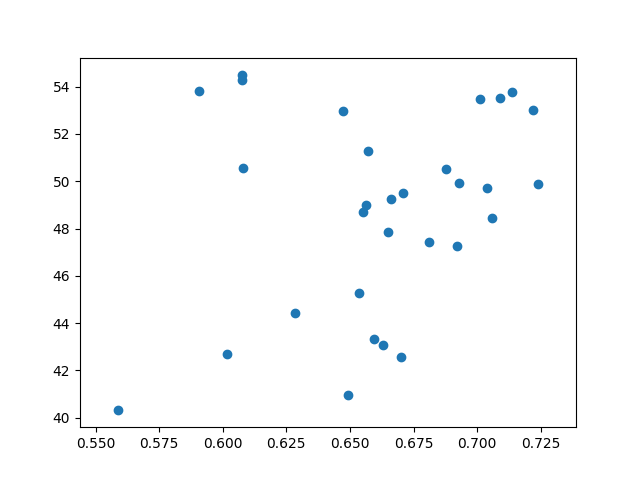
\includegraphics[width=0.45\linewidth]{evr-vs-parallelness-ldim10.png}
		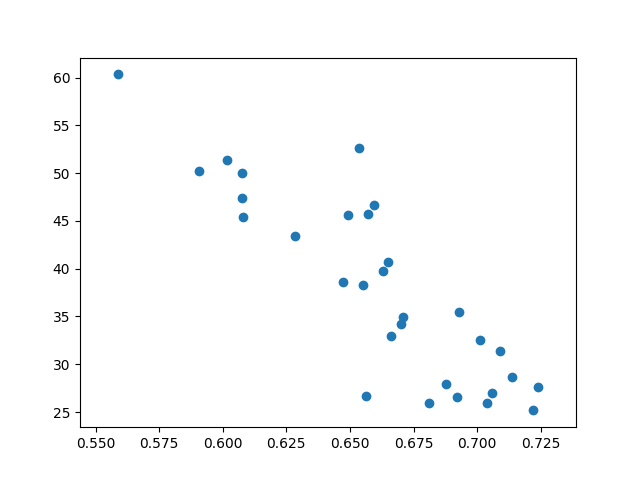
\includegraphics[width=0.45\linewidth]{evr-vs-straightness-ldim10.png}
	\end{center}
  \caption{Bal oldalon (PCA / Párhuzamosság), jobb oldalon (PCA / Átlagos szög)}\label{para2}
\end{figure}

\section{Vizualizációs eszközök ismertetése}

Elsősorban a Matplotlib nevű Python könyvtárat használjuk a grafikonok rajzolásához, ebben a fejezetben azonban nem a grafikonok stílusára, vagy azok technikai felhasználására koncentrálunk, hanem arra, hogy a kísérletek során milyen típusú adatokat ábrázolunk.

\subsection{Metrika a paraméter függvényében}

Egy kísérlet abból áll, hogy a VAE háló egy bizonyos paraméterét változtatjuk, és ennek hatását vizsgáljuk különböző metrikáinkra, veszteségfüggvényre és egyéb érdekes tulajdonságokra nézve. A kísérlet szintű ábrák ezért úgy néznek ki, hogy ezek közül egyet ábrázolunk az aktuális paraméter függvényében, például a PCA metrikát ábrázoljuk a tanítási idő függvényében. Egy ilyen ábra tehát egy egész kísérletet jellemez.

Ezeken az ábrákon mindig a vízszintes tengelyen szerepel az aktuális paraméter, a függőlegesen pedig az, amit éppen mérünk. Attól függően, hogy az adott paraméternél hogyan mintavételezünk (például, ha nagyságrendenként egy-egy adatunk van), egyes grafikonok $x$ tengelye logaritmikus skálázású is lehet. A \ref{mgraph}.~ábrán például egy háló rekonstrukciós vesztesége látható a $\beta$ paraméter függvényében.

\begin{figure}[h!]
\begin{center}
 
  
	\begin{center}
	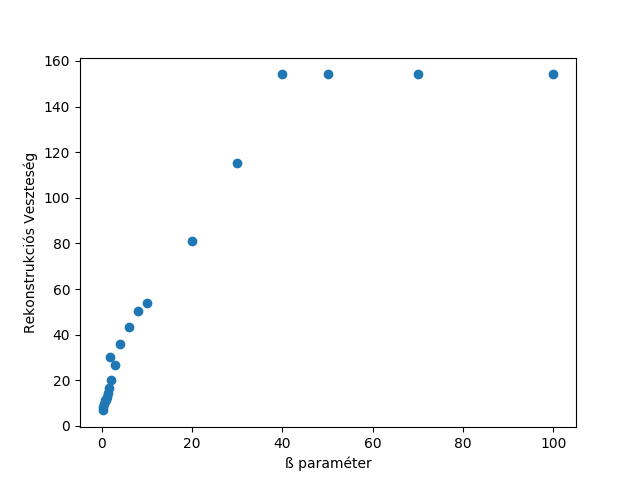
\includegraphics[width=0.75\linewidth]{metrics/vae_beta-loss.png}
	\end{center}
	
  \caption{Rekonstrukciós veszteség $\beta$ függvényében} \label{mgraph}
\end{center}
\end{figure}

\subsection{Látens vektor halmaz}

A feladat alapján az a célunk, hogy minél strukturáltabb látens teret hozzunk létre. A nehézség azonban az, hogy a látens tér valójában sok dimenziós (annyi dimenziós, ahány neuronból áll a látens réteg), ezért önmagában nem tudjuk grafikusan ábrázolni. A legmagasabb dimenzió, ami még emberi szemmel feldolgozható a $3$, ezért $n$ dimenziós ponthalmazt $3$ dimenzióssá transzformáljuk. Nyilván ekkor, ha csak a ponthalmaz nem éppen egy háromdimenziós térre esik, ez a művelet információveszteséggel jár.

A transzformációt a PCA metrikánál már ismertetett PCA algoritmussal végezzük el, amely éppen egy olyan $3$ dimenziós térre képes levetíteni a ponthalmazt, hogy a lehető legkevesebb információt veszítsünk.

Ebben a dolgozatban csak az alakzatok eltolása által kijelölt látens ponthalmazra koncentrálunk. A látens térben ezért egy bizonyos alakzat összes ($32\times32=1024$) elhelyezkedéséhez egy-egy látens pont tartozik. A könnyebb láthatóság érdekében ezen a grafikonon megszínezzünk a pontokat aszerint, hogy a hozzájuk tartozó alakzatnak mik a koordinátái. Egészen konkrétan minden pont színe két komponensből áll (zöld és piros), ahol a két szín az alakzat $x$ és $y$ koordinátájával arányosan változik, a tényleges színe pedig ezen két komponens keveréke. 

Egy ilyen grafikon tehát egy adott hálót és ponthalmazt jellemez. A \ref{m3D}.~ábrán látható példa egy ilyen grafikonra.

\begin{figure}[h!]
\begin{center} 
	\begin{center}
	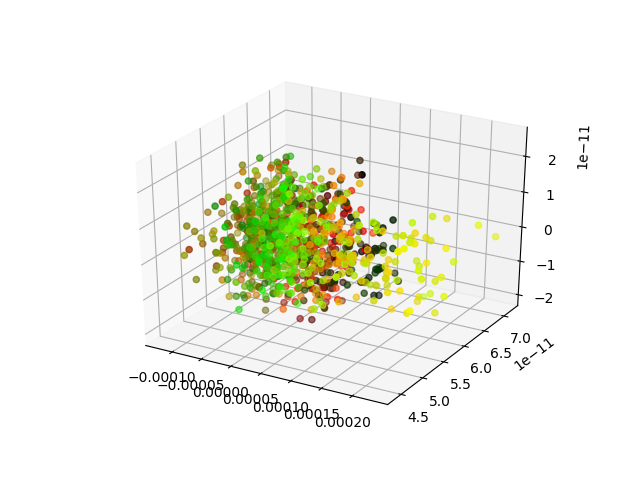
\includegraphics[width=1\linewidth]{3D-example.png}
	\end{center}
	
  \caption{Példa egy látens vektor halmaz ábrázolására}\label{m3D}
\end{center}
\end{figure}

\section{Kísérletek}

Azt vizsgáljuk a korábban definiált metrikáinkon keresztül, hogy az alábbi paraméterek hogyan hatnak a látens tér strukturáltságára. A strukturáltság azonban önmagában még nem eredményez egy jól működő hálót. Ahhoz, hogy egyáltalán az autoencoder szerepét betöltse a VAE, alacsonynak kell lennie a rekonstrukciós veszteségnek is (ezt egyszerűen ki tudjuk olvasni a tanítás során, nem kell új metrikát bevezetni hozzá), ezért a kísérleteknél vizsgáljuk az MSE-t (Mean Square Error) is. Ez egyszerűen az átlagos négyzetes hiba (a kapott és várt output között). Ezt mostantól hívjuk csak rekonstrukciós veszteségnek, hiszen ez az a mérőszám, ami azt írja le, hogy az autoencoder milyen mértékben tud rekonstruálni.

A kísérletekben tehát egy-egy paramétert változtatunk, a többit viszont változatlanul hagyjuk. A paraméterek alapértékei (amikor éppen nem változnak) a következőek:

\begin{itemize}
  \item Tanítási idő: 15 epoch
  \item Tanítási ráta: 0.0003
  \item Súly felejtés: 0.0
  \item $\beta$ hiperparaméter: 1
  \item Látens tér dimenziója: 10
  \item Háló architektúrája: konvolúciós
\end{itemize}

\subsection{Konvolúciós architektúra hatása}

A konvolúciós hálók kifejezetten képek feldolgozására alkalmasak, azonban elméletben használhatnánk sűrű hálókat is, ezek azonban mind a disentanglement, mind a rekonstrukciós feladatokban rosszabb teljesítménnyel működnek. 

A \ref{3D-dense}.~ábrán látható látens tér egy sűrű hálóhoz tartozik, és azt látjuk rajta, hogy habár a hasonló pozíciójú (pont színezésű) alakzatokhoz hasonló látens koordináták tartoznak, az ábra strukturáltsága nem közelíti meg a \ref{3D-conv}.~ábrán látható konvolúciósét.

Ezen előzetes eredmények alapján a további kísérleteinket kizárólag konvolúciós hálókkal végeztük.

\begin{figure}[h!]
\begin{center}
  
  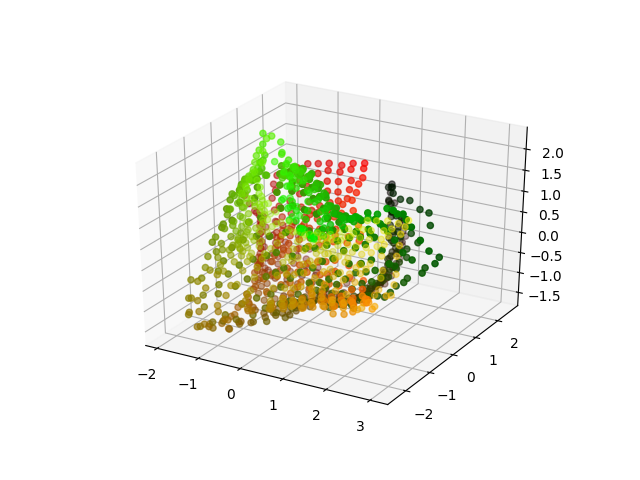
\includegraphics[width=\linewidth]{metrics/3D-dense.png}
  \caption{Sűrű háló látens tere}\label{3D-dense}
\end{center}
\end{figure}

\begin{figure}[h!]
\begin{center}
  
  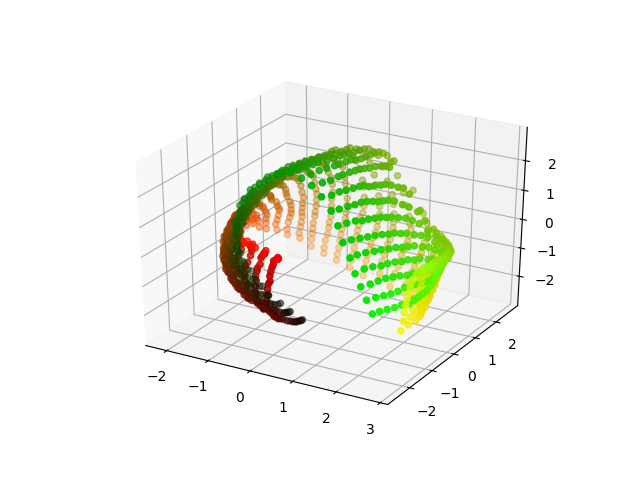
\includegraphics[width=\linewidth]{metrics/3D-epoch18.png}
  \caption{Konvolúciós háló látens tere}\label{3D-conv}
\end{center}
\end{figure}

\subsection{Tanulási idő hatása}

Ebben a kísérletben azt vizsgáltuk, hogy a tanítási idő miként hat a háló látens terének strukturáltságára. Összesen nyolcféle hálót teszteltünk, melyek kizárólag abban különböztek, hogy hány epoch-ig tartott a tanításuk. Ezek az epoch-ok a: $3, 6, 9, 12, 15, 18, 21, 24$. Ennek megvalósítására két megoldás is lehetséges: egy háló tanítását $3$ epoch-onként félbeszakítjuk és kimentjük a releváns adatokat, vagy $8$ különböző hálót tanítunk a kezdettől, és mindegyiket más-más epoch számig futtatunk. Az alábbi adatok az utóbbi megvalósításával keletkeztek.

A \ref{epoch-loss}.~ábrán láthatjuk, hogy a zajtól eltekintve a $15$ és $24$ közötti epoch számok bizonyulnak a legkevesebb veszteséggel járó paraméterezésnek. Érthető az is, hogy a rövid ($3-12$ epoch-os) tanítás még nem elegendő idő a hálónak arra, hogy hatékonyan rekonstruáljon. Lényegében tehát annyi látszik az ábrán, hogy az epoch szám növelése javítja a visszaállítási képességet.

\begin{figure}[h!]
\begin{center}
 \begin{center}
	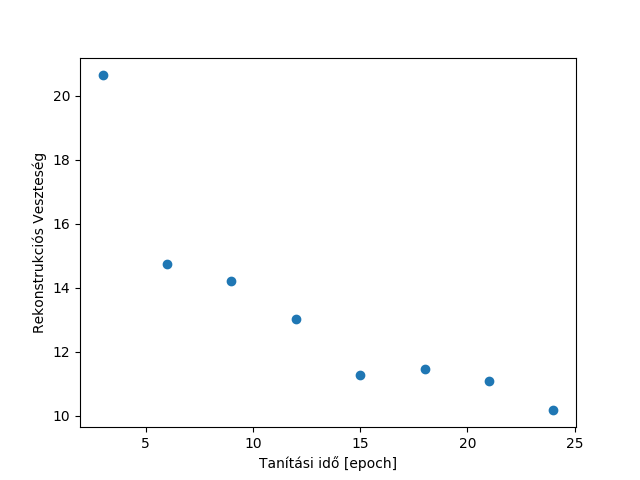
\includegraphics[width=0.75\linewidth]{metrics/vae_epoch-loss.png}
 \end{center}

  \caption{Rekonstrukciós veszteség a tanítási idő függvényében}\label{epoch-loss}
\end{center}
\end{figure}

Vizsgáljuk meg a metrikáinkat is (lásd \ref{epoch-metrics}.~ábra).  A metrikákon az látszik, hogy az egymáshoz közeli epochok esetében is extrém eltérések vannak. Ez abból adódik, hogy minden tanításhosszhoz egy külön hálót tanítottunk, ezért a véletlen is közrejátszik az eredményekben. A helyes megoldása ennek a problémának az lett volna, hogy minden kísérlet minden paraméterére több hálót tanítunk, majd a végén a kapott eredményeket átlagoljuk, erre azonban nem volt elegendő számítási kapacitás, a végeles modellek így is összesen több mint $50$ órát futottak. Ezt mellesleg technikai okokból többször is meg kellett ismétleni. 

\begin{figure}[h!]
  
  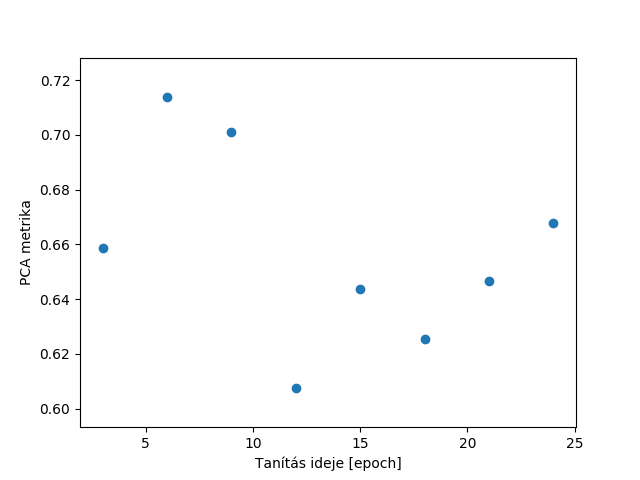
\includegraphics[width=0.5\linewidth]{metrics/vae_epoch-pca.png}
  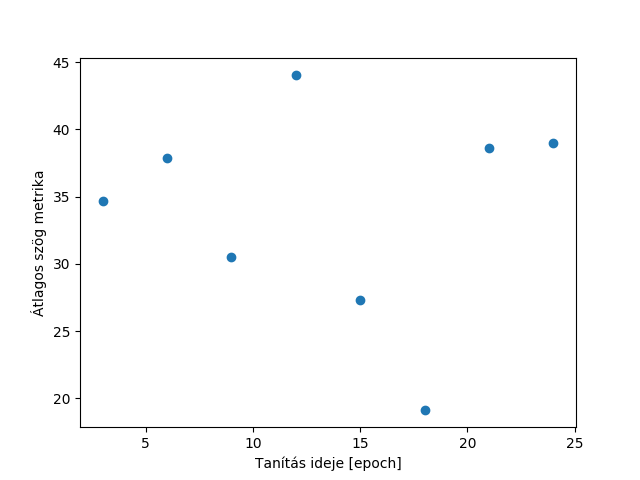
\includegraphics[width=0.5\linewidth]{metrics/vae_epoch-as.png}
  \caption{Bal oldalon a PCA metrika, jobb oldalon az Átlagos szög metrika}\label{epoch-metrics}
\end{figure}

A \ref{3D-epoch}.~ábrán látható, hogy $3$ dimenzióba vetítve, hogy néz ki egy konkrét alakzat eltolása az összes lehetséges pozícióba (összesen tehát $32\times32=1024$ darab pont van az ábrán). Az ábra a $18$ epochig futtatott hálóhoz tartozik és látszik rajta, hogy strukturáltan reprezentálja az egymáshoz képest csak egy eltolásban különböző alakzatokat. Tisztán kivehetőek szabad szemmel is az $x$ és $y$ irányú (zöld és piros) görbék, sőt még a meghajlított négyzetháló is jól látszik.

\begin{figure}[h!]
\begin{center}
 
	\begin{center}
	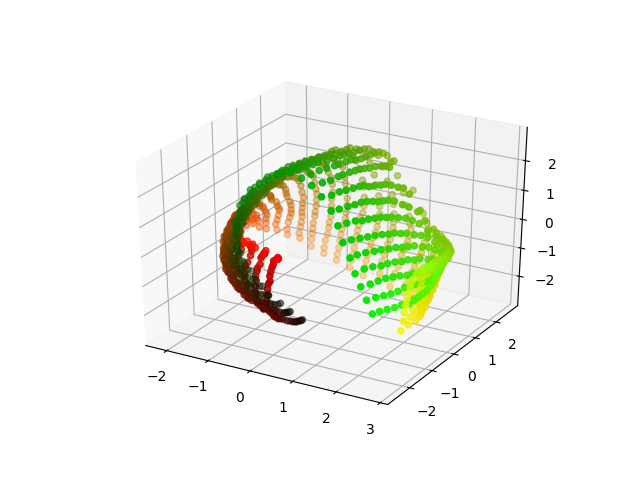
\includegraphics[width=1\linewidth]{metrics/3D-epoch18.png}
	\end{center}
	
  \caption{$18$ epoch tanítás után a látens tér}\label{3D-epoch}
\end{center}
\end{figure}

\subsection{Tanulási ráta hatása}

A tanulási ráta változtatása esetében korábban nem tapasztalt problémák merültek fel. Itt nem az történt, hogy a többszöri futtatás hiánya zajos adatot eredményezett, hanem egyszerűen egy-két paramétert leszámítva az összesre extrém méretű adatokat kaptunk, melyekből nem lehetett metrikákat számolni (egyes koordináták túlságosan nagyok lettek), sőt a nagyobb tanulási ráták esetén még a veszteségfüggvény is a végtelenbe divergált.

Ez a jelenség természetesen ismert: ha túl nagyra választjuk a tanítási rátát akkor előfordulhat, hogy a súlyokon minden batch-ben túl sokat változtatunk, ezért a veszteségfüggény alternálni fog az optimum körül, ahelyett, hogy folyonosan közelítené meg. Az ilyen módon helyes és helytelen viselkedés közti különbséget illusztrálja a \ref{para}.~ábra. Előfordulhat azonban még egy ennél rosszabb lehetőség is, amikor a veszteségfüggvény még csak nem is közelíti az optimumot, hanem a végtelenbe divergál. A $0.1, 0.3$ paraméterezésű hálóink minden bizonnyal ezért eredményeztek nagyon nagy veszteségeket.

\begin{figure}[h!]
  
  
	\begin{center}
	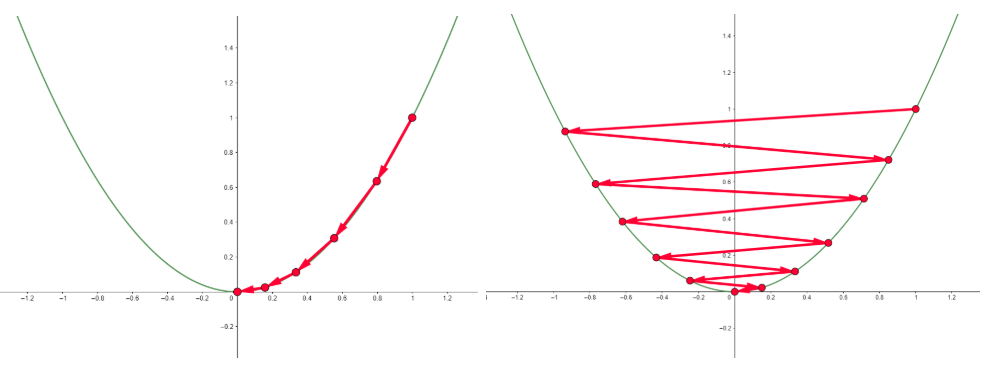
\includegraphics[width=1\linewidth]{parabolas.png}
	\end{center}
	
  \caption{A bal oldali ábrán egy kicsi, a jobb oldali ábrán pedig egy nagy tanítási ráta}\label{para}
\end{figure}



\subsection{Súly felejtés mértékének hatása}

Ebben a kísérletben a súly felejtés mértékének hatását vizsgáltuk meg összesen $11$ hálóra. A paraméter tesztelt értékei: $0.0005, 0.001, 0.002, 0.003, \dots , 0.009, 0.01$.

A \ref{wd-loss}.~ábrán láthatjuk ismét a rekonstrukciós veszteséget, az aktuális paraméter, tehát a súly felejtés függvényében. Azt tapasztaljuk, hogy a veszteségre nincs számottevő hatása a súly felejtésnek, hiszen ezekre a paraméterekre (már pedig ennél nagyobb súly felejtést nem is szokás használni) a korreláció gyenge a súly felejtés és a veszteség között. 

Érdemes megfigyelni azt is, hogy míg például az epoch számos kísérletnél a veszteségek $26$-tól $34$-ig terjedtek, addig itt mindössze egy $3.5$ pontos intervallumban helyezkednek el. Ez annyit jelent, hogy habár ránézésre véletlenszerűnek tűnnek a veszteségek, valójában arról van szó, hogy a súly felejtés lényegében nem tudja változtatni a rekonstrukciós hibát.


\begin{figure}[h!]
\begin{center}
  
  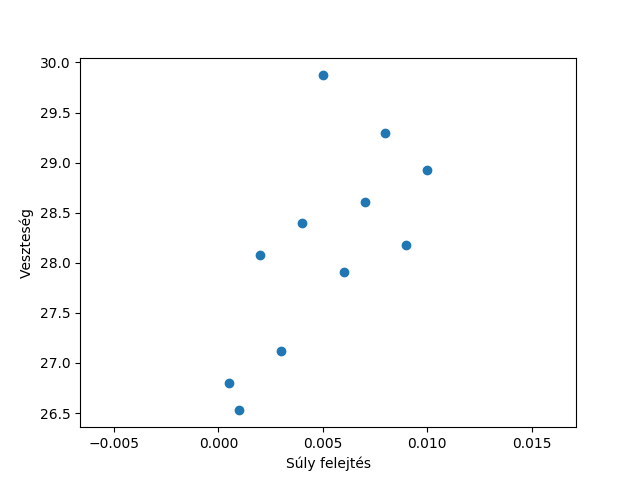
\includegraphics[width=0.75\linewidth]{metrics/vae_wd-loss.png}
  \caption{Rekonstrukciós veszteség a súly felejtés mértékének függvényében}\label{wd-loss}
\end{center}
\end{figure}

A \ref{wd-metrics}.~ábrára nézve a korábbiakhoz hasonlóan a PCA és Átlagos szög metrikák látszanak és hasonló a tapasztalat a veszteséghez: a látens tér strukturáltsága is független a súly felejtés mértékétől.

\begin{figure}[h!]
  
  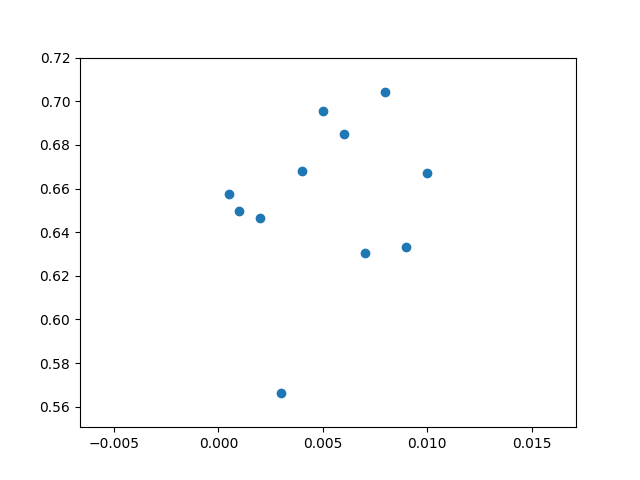
\includegraphics[width=0.5\linewidth]{vae_wd-pca.png}
  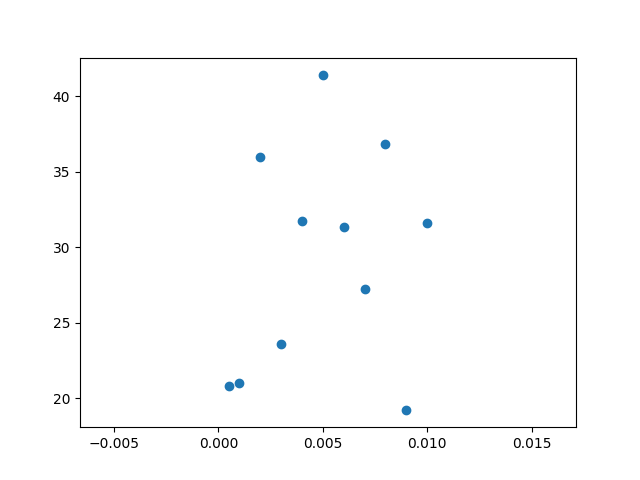
\includegraphics[width=0.5\linewidth]{vae_wd-as.png}
  \caption{Bal oldalon a PCA metrika, jobb oldalon az Átlagos szög metrika}\label{wd-metrics}
\end{figure}

Láthatjuk tehát -- legalábbis a szintetikus adathalmazunkra -- , hogy a súly felejtés mértéke sem a rekonstrukcióra sem a reprezentációra nincs jól definiálható hatással.

\subsection{$\beta$ hiperparaméter hatása}

A hagyományos VAE hálókban nem szerepel $\beta$ paraméter, csak a kiterjesztett $\beta$-VAE hálókban. Emiatt azonban nem kell teljesen megváltoztatni az alap architektúrát, mivel a VAE egy speciális változata a $\beta$-VAE-nak.

A $\beta$ paraméter -- amint azt már korábban említettünk -- azt határozza meg, hogy a látens térben rekonstrukció origóból kifele mutató és a KL divergencia origóba befelé mutató húzó erejének mi az aránya. Ha $\beta>1$ akkor a KL divergencia, ha $\beta<1$, akkor a rekonstrukciós erő dominál ($\beta=1$, akkor pedig egy hagyományos VAE hálóról beszélünk).

Ezt a paramétert számos értékre megvizsgáltuk: $0.2$-től $2.0$-ig $0.2$-esével, majd onnantól egyre ritkábban, egészen $100$-ig. A \ref{beta-loss}.~ábrán a rekonstrukciós veszteséget megtekintve azt láthatjuk, hogy lényegében a $\beta$ paraméter növelésével monoton nő, egyre kisebb mértékben és nagyjából $155$-höz konvergál. 

Ez a viselkedés teljes mértékben megfelel a várakozásoknak, hiszen $\beta$ növelése éppen azt jelenti, hogy a súlyok felülírása egyre kevésbé függ a rekonstrukciós hibától és egyre jobban függ a KL divergenciától. $\beta=40$ érték közelében éri el a háló a maximális veszteséget, tehát ez az a pont, amikor a $\beta$-VAE elveszti autoencoder jellegét. Ilyen és ennél magasabb $\beta$ értékek esetén már tehát szinte egyáltalán nem képes a háló rekonstrukcióra.

\begin{figure}[h!]
\begin{center}
  
  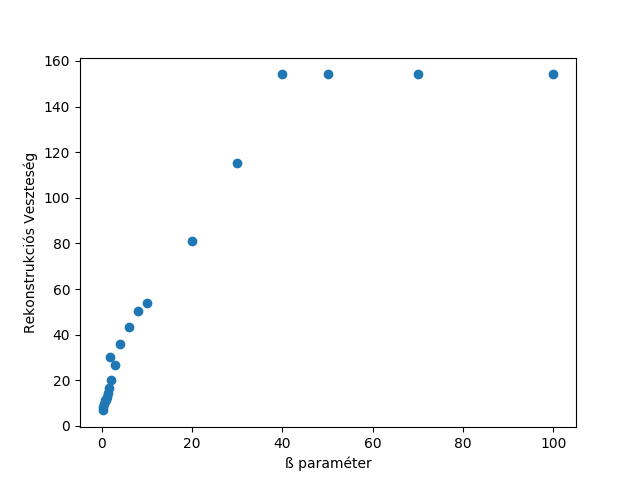
\includegraphics[width=0.75\linewidth]{metrics/vae_beta-loss.png}
  \caption{Rekonstrukciós veszteség a $\beta$ hiperparaméter függvényében}\label{beta-loss}
\end{center}
\end{figure}

Ha egy megfelelő reprezentációt keresünk, akkor természetesen az is szükséges, hogy az adatokat egyáltalán rekonstruálni képes legyen a háló. Tekintsük meg a \ref{beta-pca}.~ábrán a PCA metrikát minden $\beta$-ra, ahol ugyebár a magas értékeknek tulajdonítunk strukturált látens tereket. Az átláthatóság kedvéért az ábra $\beta$-t ábrázoló tengelye logaritmikus skálázású.

A veszteségfüggvény beláttuk, hogy a nagyon magas $\beta$-k körében értelmetlen vizsgálódni, azonban a PCA metrika mutat két kiugró pontot, mely nagyon jól strukturált látens teret ígér ($\beta=4$ és $\beta=8$ paraméterekre), hiszen megközelítőleg információveszteség nélkül tudjuk a négyzetrács görbéinek pontjait $10$ dimenzióban egy egyenesre vetíteni (más szóval a PCA metrika majdnem $1$).

\begin{figure}[h!]
\begin{center}
 
  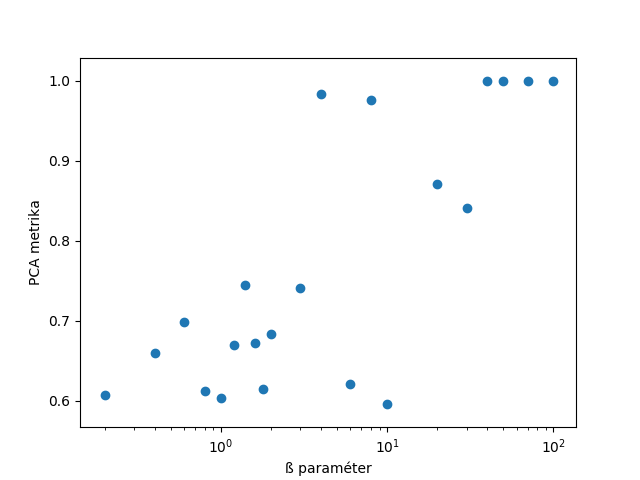
\includegraphics[width=0.75\linewidth]{metrics/vae_beta-pca-log.png}
  \caption{PCA metrika} \label{beta-pca}
\end{center}
\end{figure}

Lássuk tehát, hogy ezen két háló látens tere hogyan mutat $3$ dimenzióba vetítve (lásd \ref{3D-b4} és \ref{3D-b8}.~ábrák). A két ábra valójában nagyon hasonlít egymásra, a különbség nagy része az, hogy a vetítés során más lett az orientációjuk, a $\beta=4$-es ábrán azonban jobban látszik a struktúra.

Tisztán kivehető az alakzatmátrixhoz tartozó négyzetrács, azt is látjuk, hogy az egyik tengely mentén meg van hajlítva. A másik tengely esetében viszont teljesül az az elvárásunk, hogy egy $1$ dimenziós tulajdonságot (az alakzat $x$ koordinátáját) a látens térben egy $1$ dimenziós ponthalmaz, egy egyenes reprezentáljon. A rátekintési szögtől eltekintve éppen ezt figyelhetjük meg a $\beta=8$-as ábrán is. A látens pontok tehát olyan mértékben strukturáltan helyezkednek el, hogy már egy ilyen ábra alapján is fel tudjuk ismerni az $x=4$ koordinátájú alakzatokat.

\begin{figure}[h!]
\begin{center}
 
  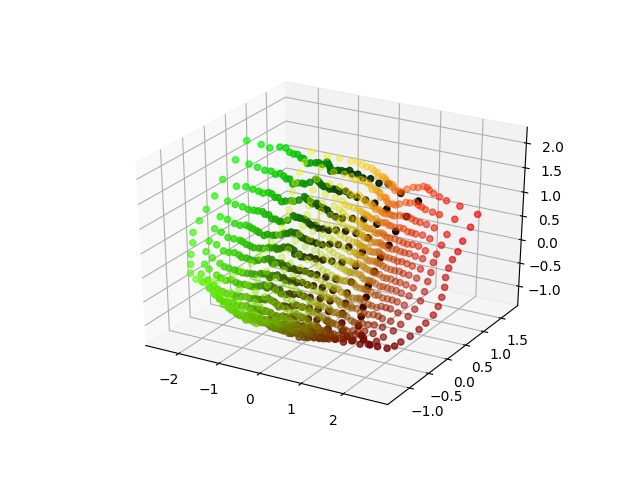
\includegraphics[width=\linewidth]{metrics/3D-b4.png}
  \caption{$\beta=4$} \label{3D-b4}
\end{center}
\end{figure}
\begin{figure}[h!]
\begin{center}
 
  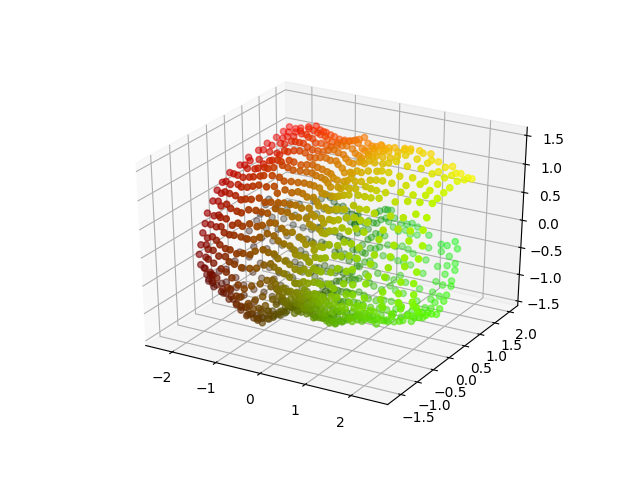
\includegraphics[width=\linewidth]{3D-beta8.png}
  \caption{$\beta=8$} \label{3D-b8}
\end{center}
\end{figure}

A reprezentáció azonban még ennél is hatékonyabb. A \ref{b4-splice}.~ábrán $10$ darab grafikon látható függőlegesen elhelyezve. Mindegyik grafikon egyetlen látens neuron aktivációjának változását ábrázolja az input kép $x$ koordinátájának függvényében. A másik, $y$ tengely értéke konstans $16$ (tehát a középső soron iterálunk végig). Ezt a műveletet pedig -- ahogy a metrikák esetében is -- sokféle alakzat, méret, orientáció hármasra elvégezzünk, és az eredményeiket átlagoljuk. Ezeket látjuk a grafikonokon. 

Azt tapasztaljuk, hogy lényegében egy konkrét neuron, a $9$. (alulról a második) az egyetlen, amely aktivációja lényegesen megváltozik, amikor az $x$ koordinátát változtatjuk. Eközben az összes többi neuron változatlan aktivitást mutat, kivéve az $5.$-et amely kis mértékben, de változtatja az értékét. A $9$. neuron ráadásul nem is véletlenszerűen változik, hanem szigorúan monoton csökken, közel lineárisan az $x$ koordináta növelésével.

Ebben a példában tehát azt látjuk, hogy a látens tér $9$. koordinátája közvetlenül és önállóan reprezentálja  az alakzatok $x$ koordinátáját, lényegében fordítottan arányos vele.

\begin{figure}[h!]
\begin{center}
  
  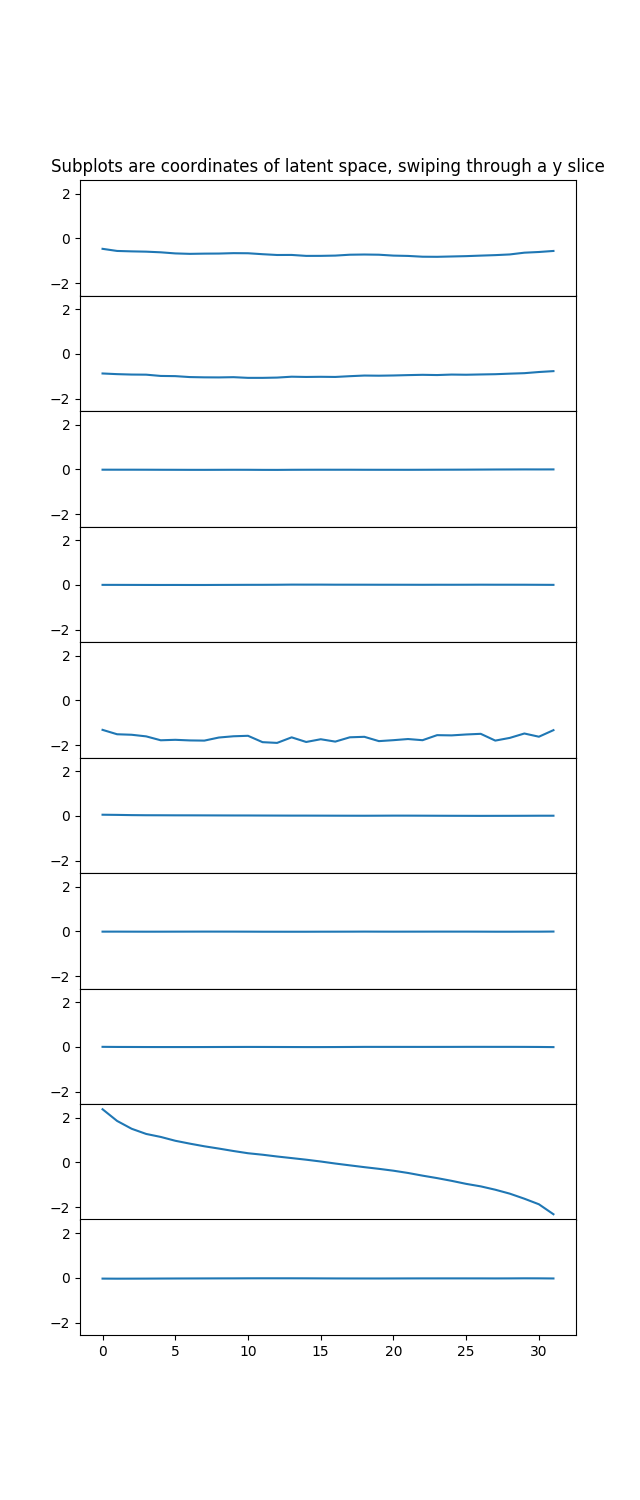
\includegraphics[width=0.5\linewidth]{slice_y16_all_coordsb4.png}
  \caption{látens neuronok használata, $\beta=4$}\label{b4-splice}
\end{center}
\end{figure}

A \ref{b100}.~ábrán a gyakorlatban is láthatjuk, hogy a magas PCA érték ellenére, miért használhatatlan a $\beta=100$-as háló.  Ahhoz hogy ezt megértsük a PCA metrika definícióját kell használnunk. Akkor magas az érték, ha a ponthalmaz minimális veszteséggel vetíthető egy egyenesre, a veszteség pedig a vetítések távolságának valamilyen aggregált értéke. Az ábrára tekintve azonban azt látjuk, hogy a teljes ponthalmaz kiterjedése kevesebb mint $10^{-10}$ ($\beta=4$-re ez az érték $3$ körüli). Ezért bármilyen origót metsző egyenesre kis veszteséggel rávetíthetőek a pontok, hiszen már lényegében az origó pontjában tömörülnek. A PCA metrika tehát ilyen esetben garantáltan az $1$ hez fog tartani, és nem hordoz magában hasznos információt.

\begin{figure}[h!]
\begin{center}
  
  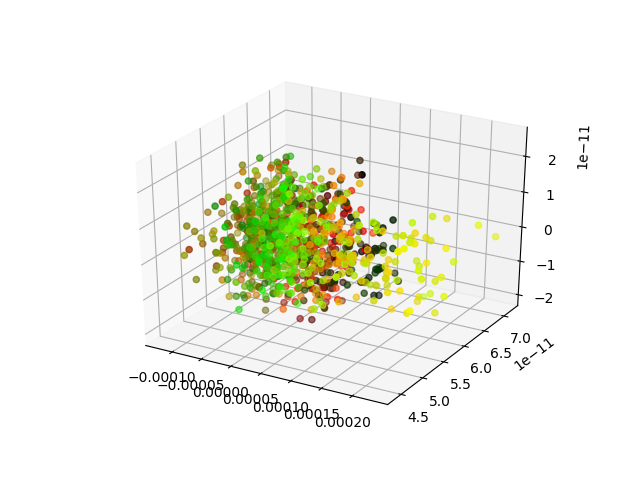
\includegraphics[width=\linewidth]{3D-beta100.png}
  \caption{$\beta=100$}\label{b100}
\end{center}
\end{figure}


Az is várható természetesen, hogy a pontok $\beta=100$-nál az origóban sűrűsödnek, hiszen ekkor a KL divergencia, azaz az origóba húzó erő dominál.

Jól strukturált látens terek esetében értelme van a látens pontokat vektorként kezelni, melyek összegezhetőek és kivonhatóak egymásból. Az \ref{interp}.~ábrán négy kép látható. Mindegyik kép bal felső sarkában $3$ bázis kép van kirajzolva, melyek a tényleges adathalmazból származnak. A kép maradék része egy négyzetrács, melynek bal felső ($\vec{A}$), jobb felső ($\vec{B}$) és bal alsó ($\vec{C}$) sarkaiban ezen három adatképnek a rekonstrukciója látható. A képen látható összes többi alakzat az $\vec{AB}$ és $\vec{AC}$ vektorok lineáris kombinációja $\vec{A}$-hoz hozzáadva, tehát $\vec{A}+\nu\vec{AB}+\mu\vec{AC}$ vektorú látens pontból generált kép. $\nu$ és $\mu$ a kis képek koordinátájával egyenletesen változik $0$ és $1$ között, vagyis a jobb alsó kép éppen az $\vec{A}+\vec{AB}+\vec{AC}$ koordinátájú látens pontból generálódott. 

Ha a reprezentációnk elég strukturált, akkor egy két látens pont közötti vektor egy transzformációként értelmezhető. Ezeken az ábrákon például az $\vec{AB}$ vektor a bal felső sarokból jobb felső sarokba eltolás transzformációját jelöli. Hasonlóan az $\vec{AC}$ vektor egy $y$ irányú transzformációt ír le. Ha pedig a két vektor összegét tekintjük, akkor jogosan várhatjuk el azt, hogy az általa leírt transzformáció a két transzformáció egymás után való elvégzését fogja jelölni. A gyakorlatban tehát egy a jobb alsó sarokban elhelyezkedő négyzetet kellene látnunk a jobb alsó képen.

A \ref{interp}.~ábrán látható négy rész ábra mind a fentiek alapján generálódik, mindössze annyiban különböznek, hogy más $\beta$ paraméterű ($\beta=0.2, 2,3,6$) hálók látens terét mutatják be. 

\begin{figure}[h!]
\begin{center}
  
  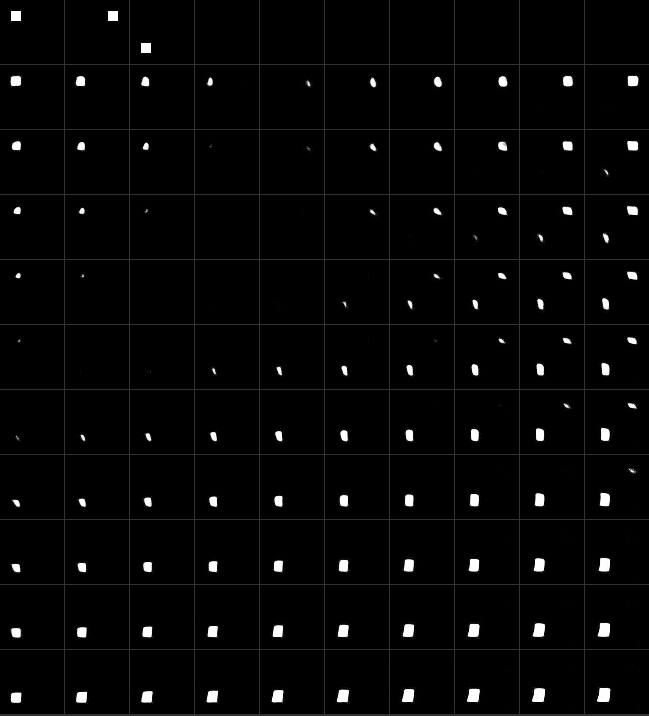
\includegraphics[width=0.49\linewidth]{metrics/interp02.png}
  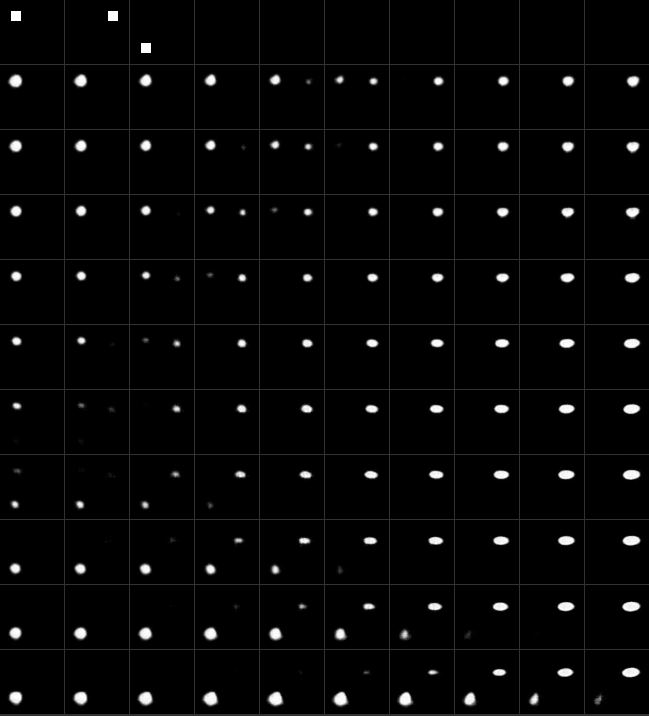
\includegraphics[width=0.49\linewidth]{metrics/interp-2.png}
  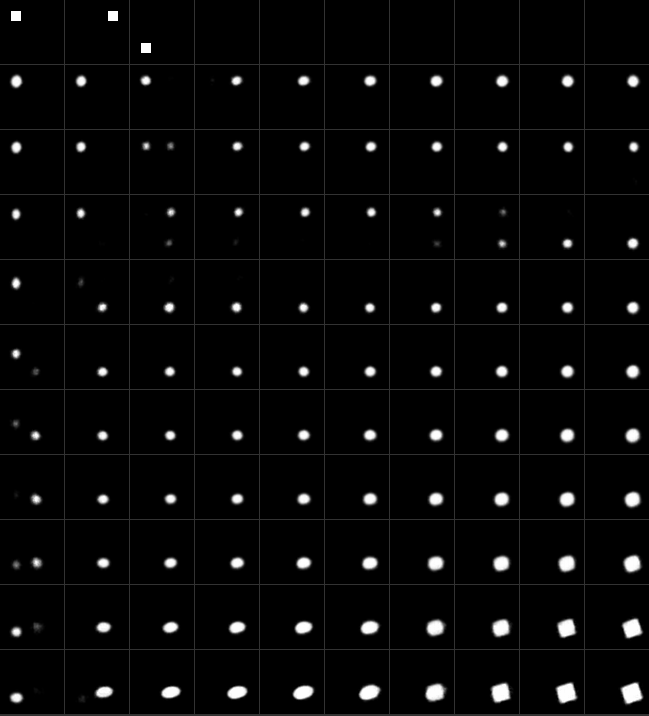
\includegraphics[width=0.49\linewidth]{metrics/interp3.png}
  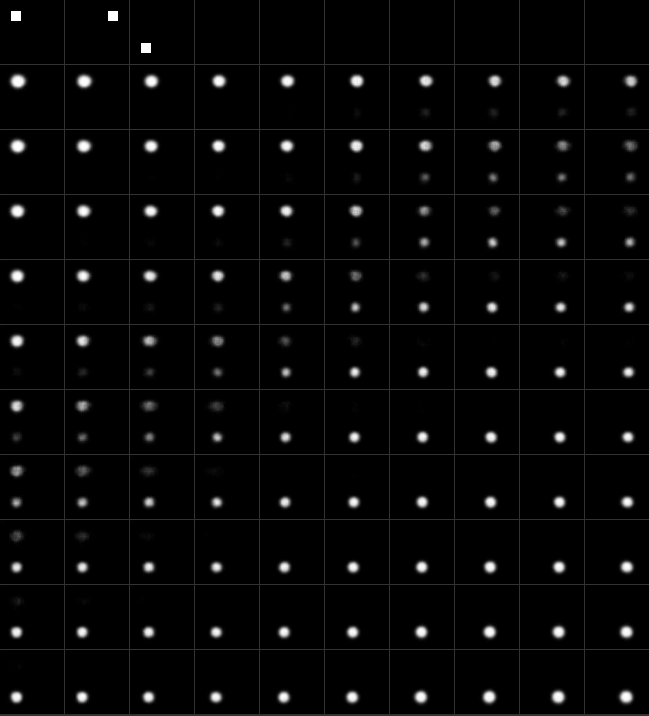
\includegraphics[width=0.49\linewidth]{metrics/interp-6.png}
  \caption{Bal felső: $\beta=0.2$, jobb felső: $\beta=2$, Bal alsó: $\beta=3$, jobb alsó: $\beta=6$.}\label{interp}
\end{center}
\end{figure}

A $\beta=0.2$ esetben azt látjuk, a három input kép sikeresen rekonstruálódik, azonban a két eltolási transzformáció összege (jobb alsó kis kép) szinte megegyezik a $\vec{C}$ vektorral, ami arra utal, hogy a látens térben $A$ és $B$ túlságosan közel van egymáshoz. Azt azonban legalább megtanulta a háló, hogy az $A, B$ és $C$ látens pontok mint négyzeteket ábrázolnak, ezért a $4$. pontnak is négyzetnek kell lennie. Megfigyelhető továbbá a képek között egy olyan zóna is, ahol a háló üres képeket rajzol. Ez a $\beta$ alacsony értékéből adódik, mivel $\beta=0.2$ az origóból kifelé ható erő dominál, ezért a tanító adatpontok távol kerülnek egymástól és a térben lehetnek olyan részek, melyek semmilyen tanító adatponthoz nem esnek közel. A hálónak tehát nincsen tapasztalata arról, hogy az ilyan látens vektorokhoz milyen képet kell generálnia, üres képeket ad.

A $\beta=2$-es ábrán tulajdonképpen a $0.2$-es ábra problémái láthatóak, viszont az előnyei nélkül, tehát a háló nem tanulta meg a transzformációt, viszont már az input képeket is csak részben képes rekonstruálni (jó pozícióba rajzolja, jó méretben, az alakzat körvonala azonban már nem vehető ki), az összeg helyére pedig már kifejezetten hibásan, ellipszist rajzol.

$\beta=3$-nál jön el az a pont (a vizsgált $\beta$-k közül), ahol a háló már képes a két transzformációt egymás után elvégezni, hiszen láthatjuk, hogy a jobb alsó képen valóban a jobb alsó sarokba rajzol négyzetet. Az, hogy a jó pozíció mellett még az alakzatot is helyesen négyzetnek rajzolja a véletlen műve lehet, mivel a háló már egy ennél jelentősen egyszerűbb feladatot a rekonstrukciót sem tudja elvégezni (legalábbis az alakzat formáját tekintve), mivel az $A, B$ és $C$ sarkokban köröket látunk. Ez nem feltétlenül jelenti azt, hogy a háló nehezen különbözteti meg a négyzeteket a köröktől, inkább azzal indokolható a jelenség, hogy a kör alakzat kevés információ rendelkezésre állása esetén bármilyen alakzatra jó tipp a hálónak, kevés lesz az átlagos veszteség. A kör forma tehát inkább egy megforgatott négyzet vizuális kiátlagolásából adódik, mint a kör típusú adatból.

$\beta=6$ esetén ennek a tendenciának a folyatása látható, itt már minden képen csak körök láthatóak. Transzformációs képesség szempontjából azonban minden korábbinál jobban viselkedik ez a háló, elég csak a legalsó sorra nézni, ahol szinte egy folytonos átmenet látható $x=1$-től az $x=31$ koordinátáig.

Ez a négy ábra jól mutatja a $\beta$-VAE működését, látszik ahogy $\beta$ növelésével egyre csökken a rekonstrukciós képesség, azonban eközben a látens tér egyre strukturáltabb, ezért képes a transzformációkat értelmezni. Az is látható továbbá, hogy a háló többi paraméterei ilyen értékekkel semmilyen $\beta$-ra sem eredményeznek egy olyan hálózatot, amely ezt a két képességet egyszerre teljesítik.



A $\beta$ hiperparaméterrel tehát a VAE és $\beta$-VAE hálók esetében mindenképp érdemes foglalkozni, ezzel a paraméterrel lehet finomhangolni azt, hogy mennyit szeretnék elengedni a rekonstrukcióból a tér strukturáltsága értekében és fordítva. A különböző adathalmazok és felhasználási célok határozzák meg egy-egy konkrét esetben, hogy mennyire érdemes választani $\beta$-t.

\subsection{Látens tér dimenziójának hatása}

A látens tér dimenziójának hatását is megvizsgáltuk néhány esetre ($6, 8, 10, \dots , 20,$ $30, 40, 50$), melyek veszteségfüggése a \ref{ldim-loss}.~ábrán látható. Itt gondolhatnánk azt, hogy a háló szűk keresztmetszetének (a látens tér dimenziójának) növelése javítja a rekonstrukciót, hiszen a generátornak több adat áll rendelkezésre, azonban ha csak ezt a paramétert növeljük, akkor ez éppen hogy megnehezíti a visszaállítást. Ugyanannyi információból egy komplexebb hálót kell építenie.

A veszteség diagramon is ez látszik, tehát ahogy növeljük a látens tér dimenzióját, úgy nő a veszteség is. Az $50$-es látens dimenzió esetében a kevés veszteség vélhetően csak egy szerencsés kezdetleges súly kiosztásnak köszönhető, azonban a $6$ és $8$ méretű látens tereknél így sem ér el jobb eredményt a rekonstrukció terén. 

Nyilván a látens tér méretét nem lehet akármeddig csökkenteni a rekonstrukció javítása érdekében, hiszen egy $1$ neuronból álló szűk keresztmetszet már biztosan nem tudna elkódolni egy $64\times64$-felbontású képet, legfeljebb akkor, ha minden pixel egyszerre változna. A mi adathalmazunk nem túl komplex, de ennél lényegesen bonyolultabb. Ahogy az a mellékelt címkékből is látszik, a Dsprite adathalmaz egy adatpontját $5$ számmal tudjuk leírni, mely az alakzatok $5$ független tulajdonságát jelöli.

A $\beta$ paraméteres fejezetben láttunk egy példát arra, hogy egy folytonos tulajdonság leírására elegendő mindössze $1$ neuron a látens rétegben (lásd. \ref{b4-splice}). Ideális esetben a látens tér dimenziója és a tulajdonságok száma között bijekció van. A látens teret ezért $5-6$ dimenziósnál kevesebbnek nincs értelme választani. A \ref{b4-splice}.~ábrához hasonlóan $5$ tulajdonság nem fog $5$ neuronnál lényegesen többet igénybe venni, $30$ neuron esetében várhatóan $20$-at szinte egyáltalán nem használ, ezért a felesleges látens neuronok csak egy zajt, potenciális hiba lehetőséget visznek a rendszerben, ami megnehezíti a rekonstrukciót.

\begin{figure}[h!]
\begin{center}
 
  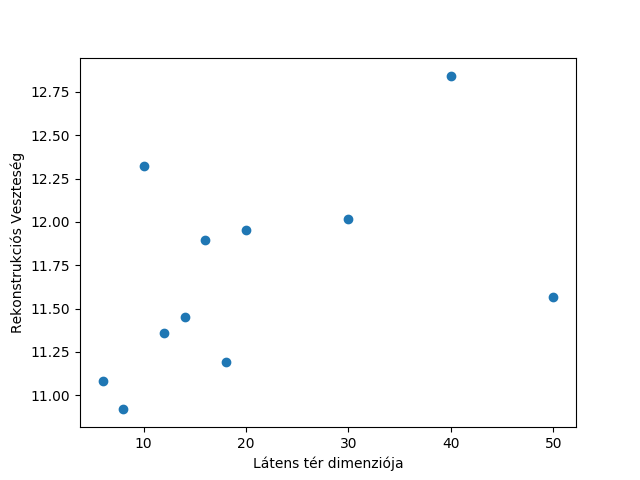
\includegraphics[width=0.75\linewidth]{metrics/vae_ldim-loss.png}
  \caption{Rekonstrukciós veszteség a látens tér dimenziójának függvényében} \label{ldim-loss}
\end{center}
\end{figure}

Nézzük meg az átlagos szög metrikánkat is ezekre az adatokra a \ref{ldim-metrics}.~ábrán. Itt is egy romló tendenciát látunk a dimenzió növelésekor, amit éppen ugyanaz magyaráz meg mint a veszteséget: hiába növeljük a látens tér méretét, egy idő után a háló akkor sem fog több neuront igénybe venni, mert a kódolandó információ mértéke változatlan. 

\begin{figure}[h!]
\begin{center}
  
  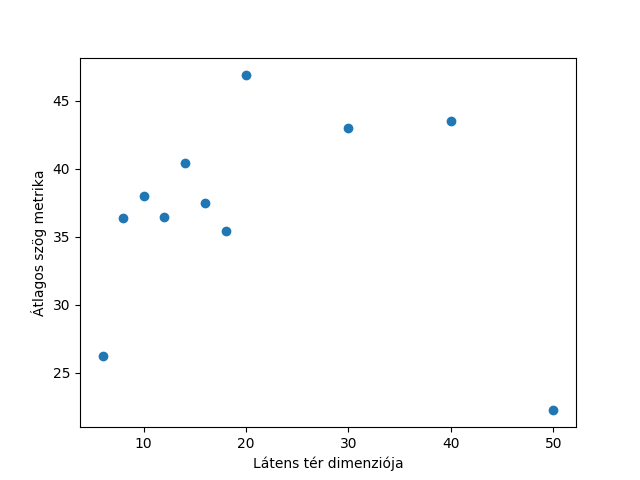
\includegraphics[width=0.75\linewidth]{metrics/vae_ldim-as.png}
  \caption{Átlagos szög metrika}\label{ldim-metrics}
\end{center}
\end{figure}


\chapter{Összefoglalás, lehetőségek}

Az eredményeket tekintve látszik, hogy mely paraméterek milyen mértékben hatottak a reprezentációra. A $\beta$ paraméter megfelelő megválasztásával láttuk, hogy nagyon letisztult látens tereket is kaphatunk. ahol szabad szemmel ráismerhetünk az adathalmaz bizonyos elemeire.

A modellek kiértékelése során számos problémával szembesültem, például azzal, hogy egyetlen betanítás után egy háló meglehetősen zajos eredményeket produkál nem csak a saját metrikáimra nézve, a veszteségfüggvények alapján is. A hálók tanítása során keletkező zajt azonban csak extra teljesítménnyel lehetett volna kiküszöbölni, minden háló többszöri véletlen inicializációval való futtatásával. Ez tehát egy potenciális javítási lehetőség.

Ahol csak tudtam, próbáltam tompítani a zajt sokszori futtatással, majd átlagolással például a metrikák számolásánál minden érték úgy keletkezik, hogy sok különböző alakzatot eltolok, majd a rajtuk kiszámolt metrikákat átlagolom. 

Egy másik, problémának nem nevezhető jelenség, hogy bizonyos paraméterek teljesen irrelevánsnak bizonyultak a látens tér strukturája szemponjából, pélidául a súly felejtés.

Konvolúciós hálók révén egyéb paraméterek reprezentáció-hatását is meg lehetne vizsgálni: padding, stride, filterek száma, a háló rétegeinek dimenziói és száma.

Tesztelhető lenne ezek mellett az "Understanding disentangling in $\beta$-VAE" \cite{dbvae} publikációban bemutatott módszer is, amely a úgy segíti a disentanglementet, hogy közben a rekonstrukciós képesség nem romlik olyan mértékben, mint a hagyományos $\beta$-VAE esetében.

További lehetőség lenne dolgozatban látott elemzés elvégzése más, akár nem szintetikus adahalmazokon is, mint például a Celeba adathalmaz.

\begin{thebibliography}{9}

\bibitem{ConvNet}
CS231n Convolutional Neural Networks for Visual Recognition:\\
\url{http://cs231n.github.io/convolutional-networks/}

\bibitem{Dsprite}
{Loic Matthey and Irina Higgins and Demis Hassabis and Alexander Lerchner},
\textit{dSprites: Disentanglement testing Sprites dataset},\\
\url{https://github.com/deepmind/dsprites-dataset/
} (2017)

\bibitem{VAE}
Variational Autoencoders Explained\\
\url{http://kvfrans.com/variational-autoencoders-explained/}

\bibitem{original VAE}
Variational Autoencoder\\
\url{https://arxiv.org/abs/1606.05908}

\bibitem{bvae}
Understanding disentangling in $\beta$-VAE\\
\url{https://arxiv.org/abs/1804.03599}

\bibitem{dbvae}
Understanding disentangling in $\beta$-VAE\\
\url{https://arxiv.org/abs/1804.03599}

\bibitem{original GAN}
Generative Adverarial Networks\\
\url{https://arxiv.org/abs/1406.2661}

\bibitem{tensorflow}
TensorFlow\\
\url{https://www.tensorflow.org/}

\bibitem{Keras}
Keras\\
\url{https://keras.io/}

\end{thebibliography}

%\end{document}
